\section{R\'esum\'e en fran\c cais}

\renewcommand{\sm}{Modèle standard}
%-----------------------------------------------------------------------------
%-----------------------------------------------------------------------------
%-----------------------------------------------------------------------------
\subsection*{Introduction}
\begin{figure}
	{\centering
		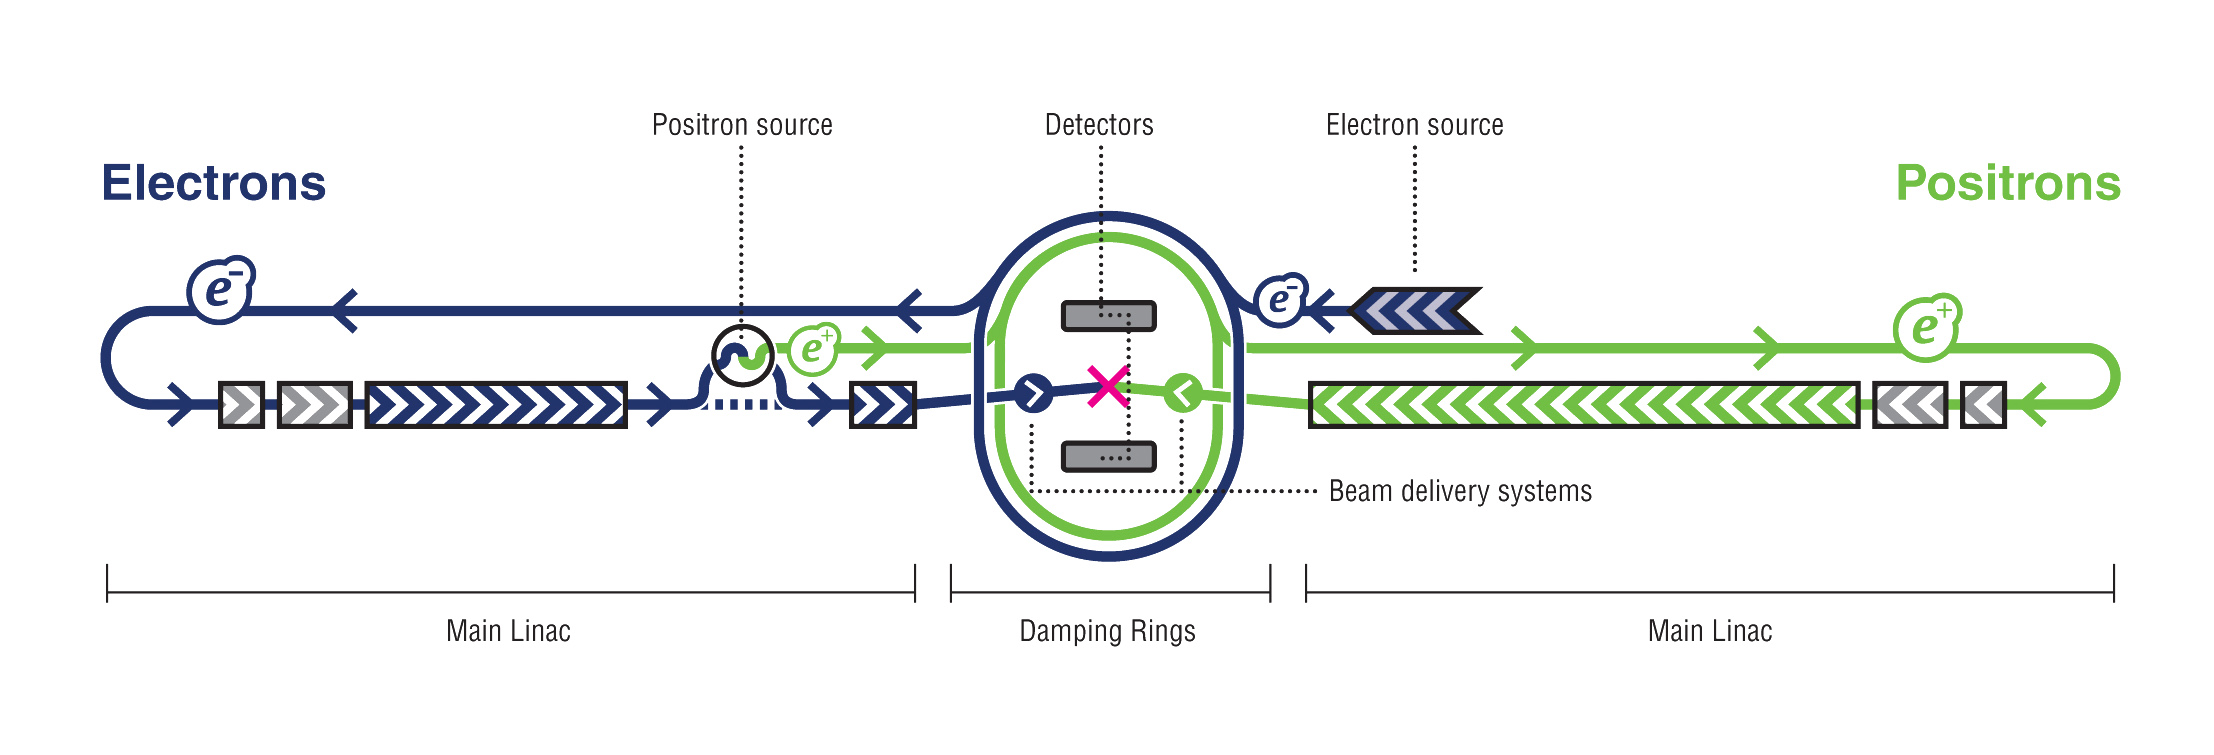
\includegraphics[width=0.95\textwidth]{graphics/ILC_scheme.jpg}
		\caption{\sl Vue sch\'ematique de l'ILC.}
		\label{fig:ILCSchemeF}
	}
\end{figure}

\begin{figure}
	\centering
	\begin{subfigure}{0.5\textwidth}
		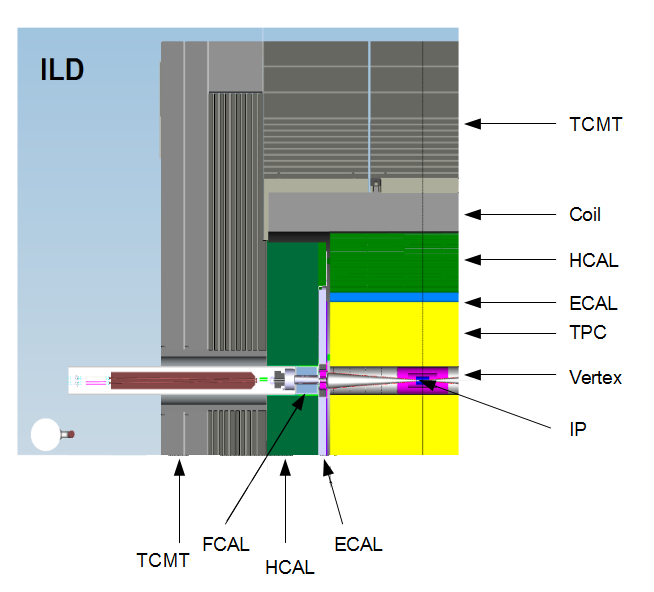
\includegraphics[width=0.95\textwidth]{graphics/ILD.png}
		
	\end{subfigure}% 
	\begin{subfigure}{0.5\textwidth}
		\centering
		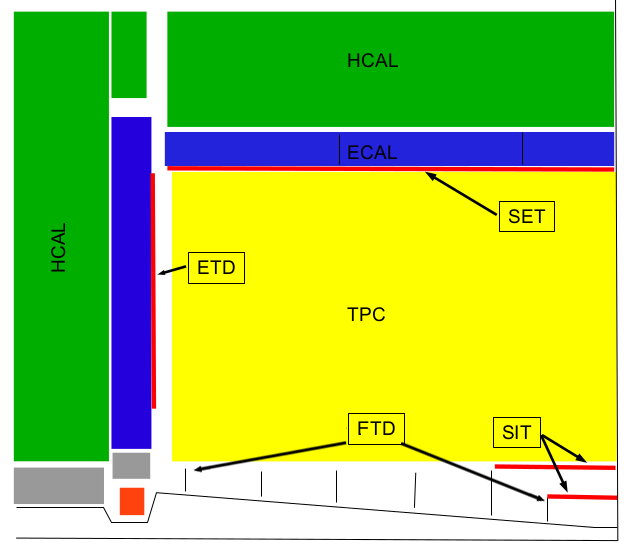
\includegraphics[width=0.9\textwidth]{graphics/ILDtracking.png}
		
	\end{subfigure}
	\caption{\sl Gauche: Vue sch\'ematique de l'ILD. Droite: Zoom sur les détecteurs internes.}
	\label{fig:ILDSchemeF}
\end{figure}
%-----------------------------------------------------------------------------
%-----------------------------------------------------------------------------
%-----------------------------------------------------------------------------
\subsection*{Calorim\`etre \'electromagn\'etique silicium-tungst\`ene hautement granulaire}

\begin{figure}[H]
	\centering
	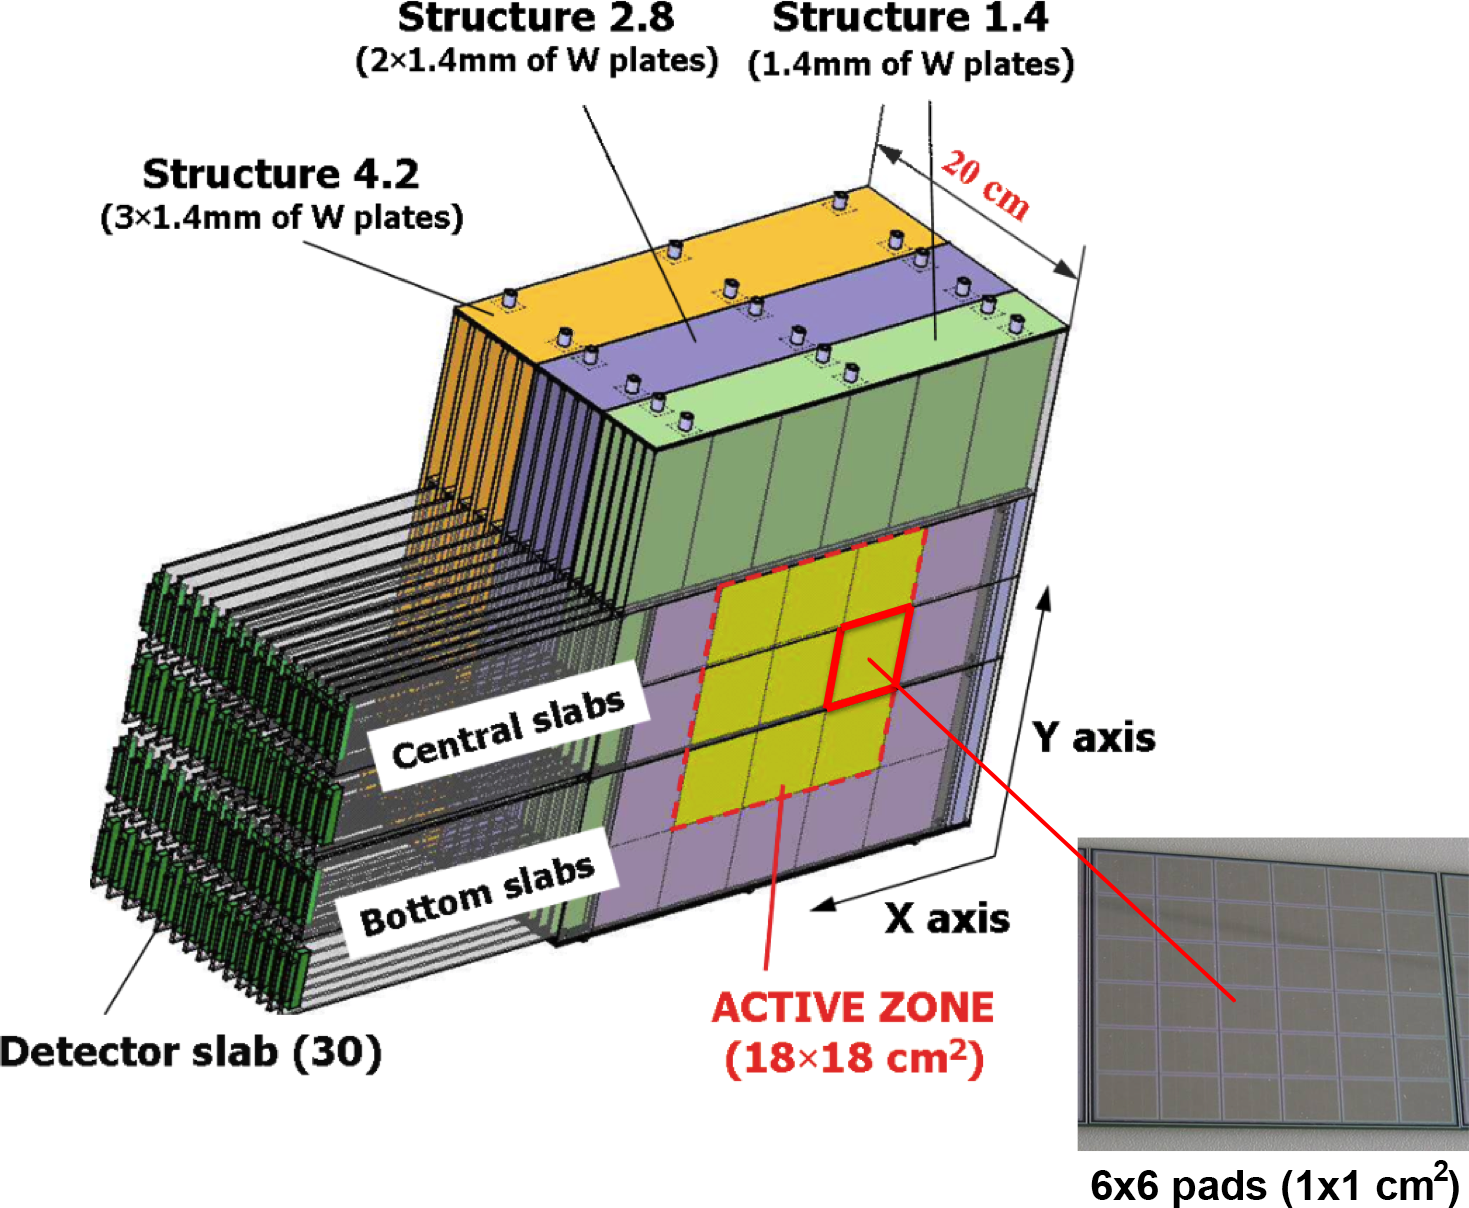
\includegraphics[width=0.55\textwidth]{ECAL/graphics/ecal-new.png}
	\caption{\label{fig:ECAL-schemeF} \sl  Vue sch\'ematique de \ecal.}
\end{figure}

%-----------------------------------------------------------------------------
%-----------------------------------------------------------------------------
%-----------------------------------------------------------------------------
\subsection*{L'algorithme de reconstruction des traces}

\begin{figure}
	\centering
	\begin{subfigure}{0.5\textwidth}
		\centering
		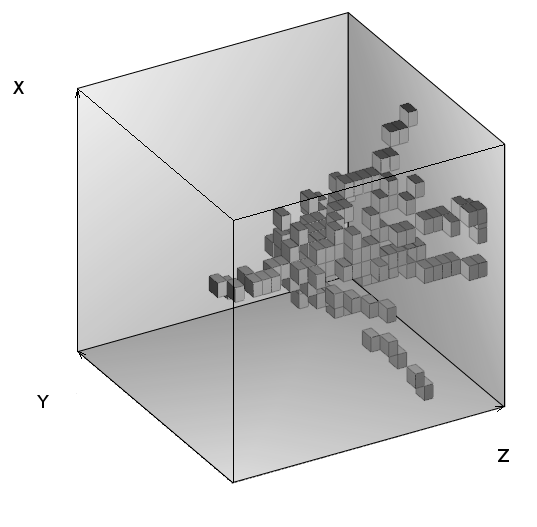
\includegraphics[width=.90\linewidth]{ECAL/graphics/before.png}
		\caption{\label{fig:beforeF} \sl avec région d'interaction.}
	\end{subfigure}% 
	\begin{subfigure}{0.5\textwidth}
		\centering
		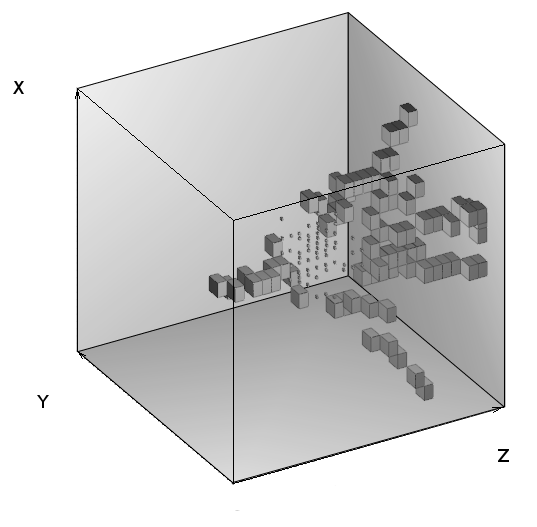
\includegraphics[width=.90\linewidth]{ECAL/graphics/after2.png}
		\caption{\label{fig:afterF} \sl sans région d'interaction.}
	\end{subfigure}
	\caption{ \sl Visualisation d'événement de l'interaction pion primaire avec 10\,GeV d'energie enregistré au FNAL 2008 avant \textit{(a)} et apr\'es suppression de la région d'interaction\textit{(b)}. }
	%Event 16-17 in Data10.root
	\label{fig:testF}
\end{figure}


\begin{figure}
	\centering
	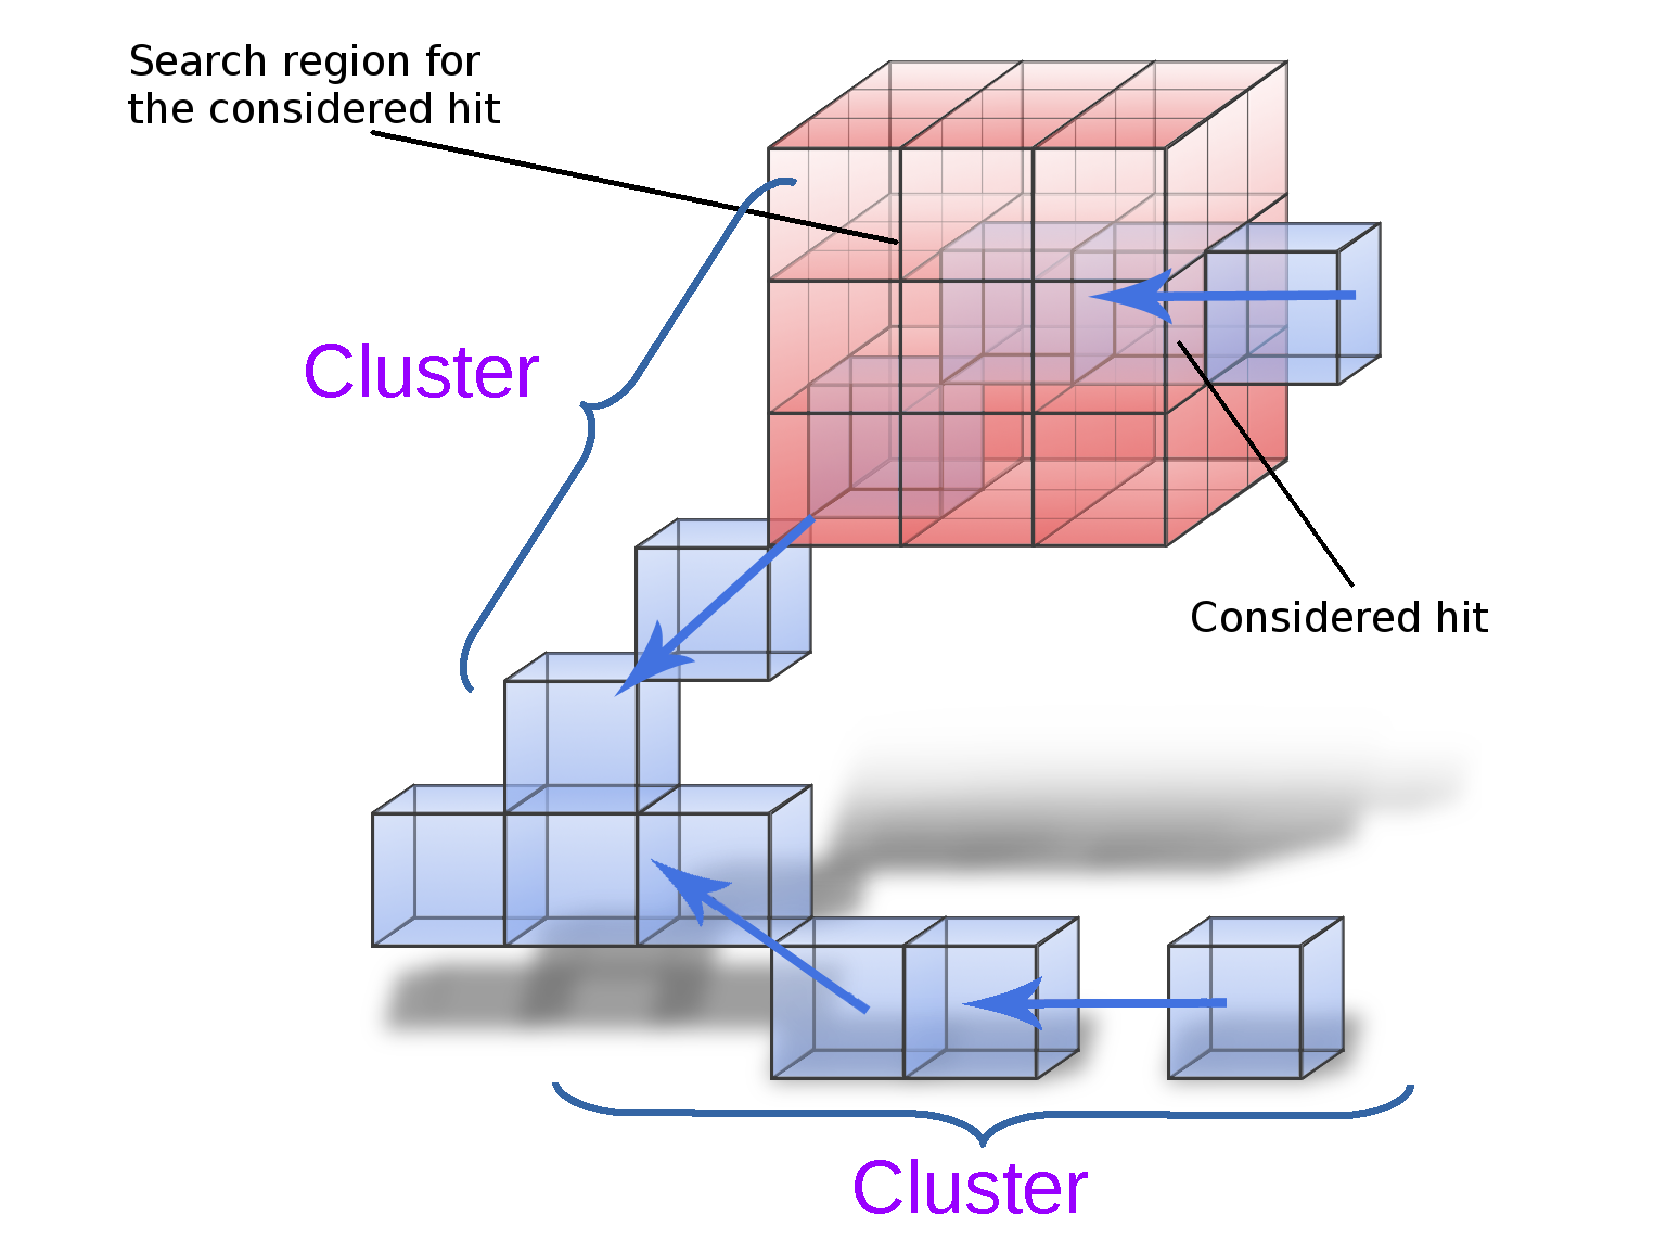
\includegraphics[width=0.55\textwidth]{ECAL/graphics/demo-v3.pdf}
	\caption{\label{fig:democlusterF} \sl Illustration de l'étape de clusterization. Les pixels actives sont représentés par des cubes bleus, et la zone de recherche pour les impacts adjacents est indiquée par des cubes rouges. Les flèches bleues indiquent la direction du flux de clusterization.}
\end{figure}

%-----------------------------------------------------------------------------
%-----------------------------------------------------------------------------
%-----------------------------------------------------------------------------

\subsection*{Comparaison des simulations avec les données réelles}



\begin{figure}
	\centering
	\begin{subfigure}{0.5\textwidth}
		\centering
		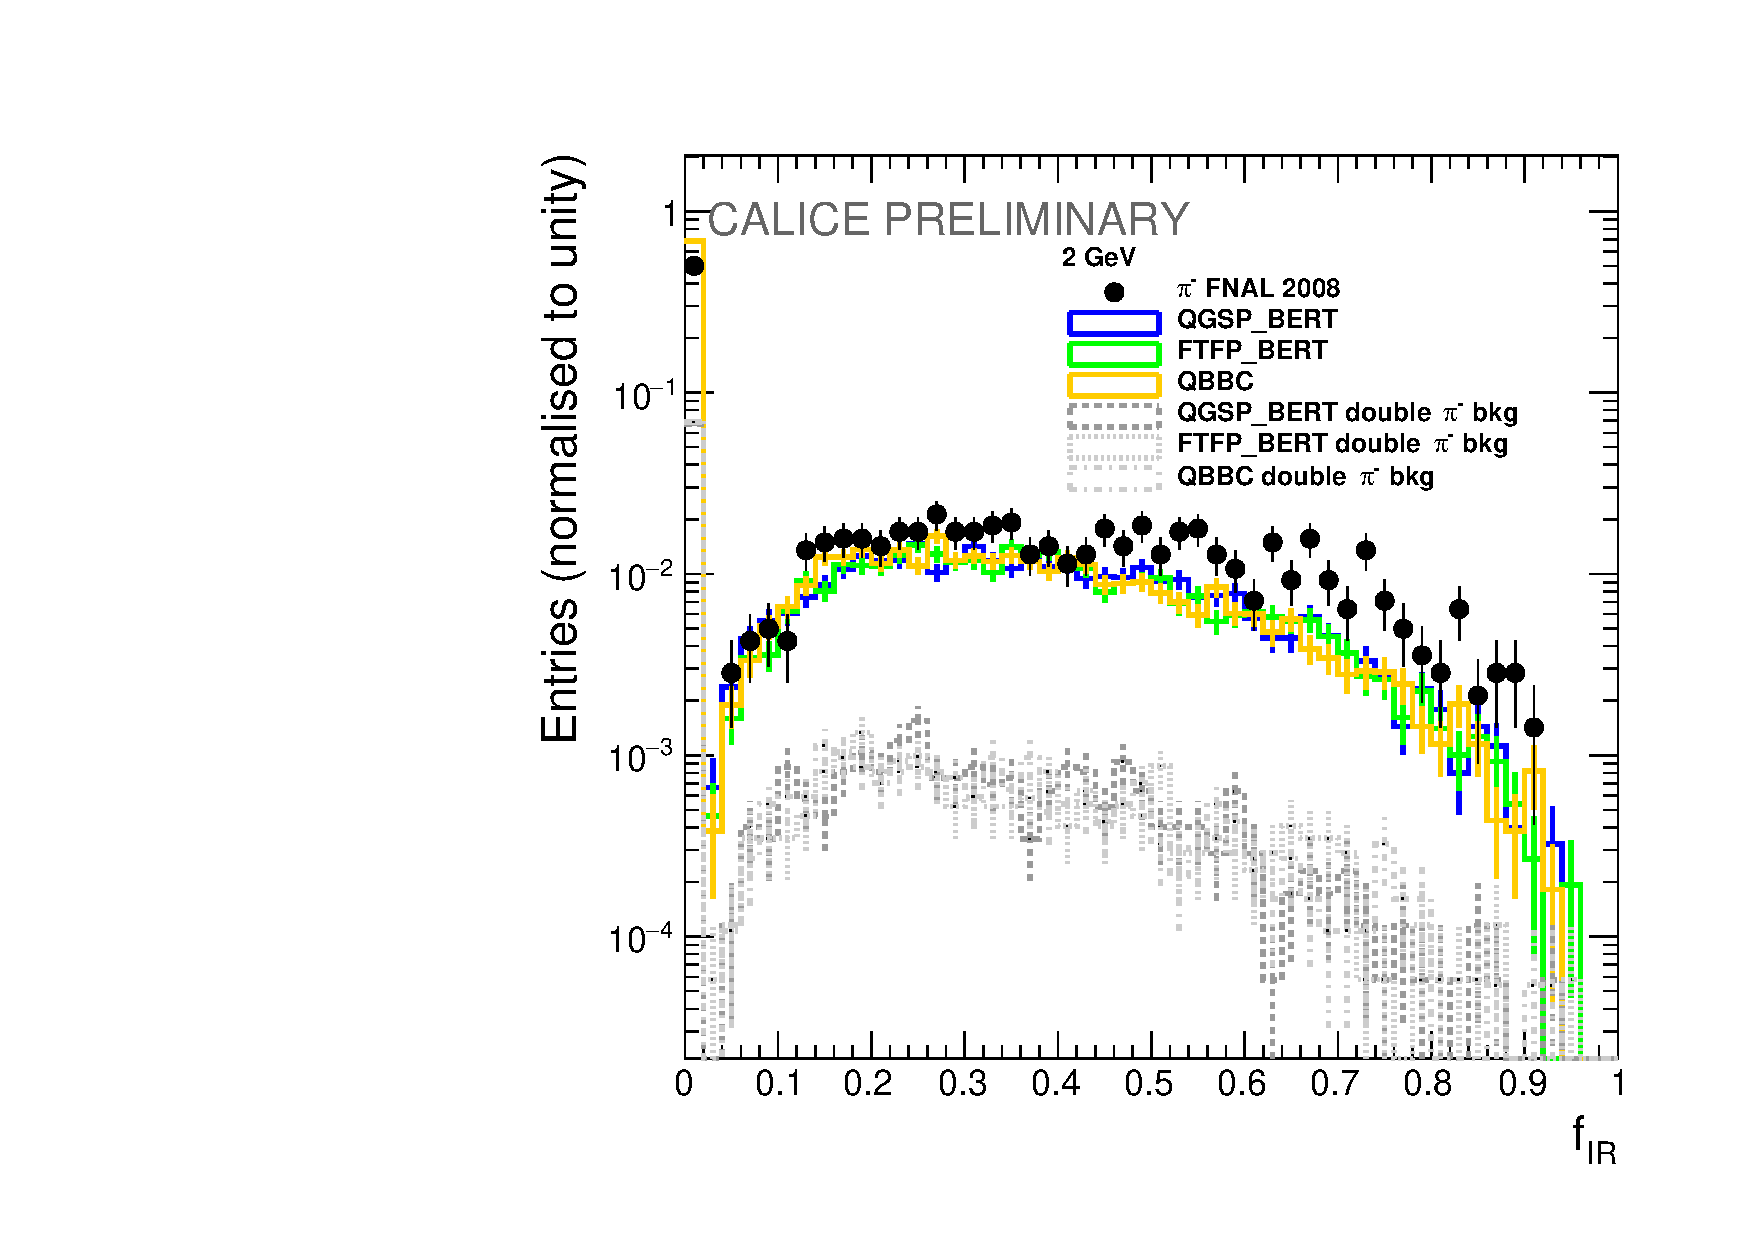
\includegraphics[width=.90\linewidth]{ECAL/plots/e-ir-2.pdf}
		\caption{\label{fig:efr2F} }
	\end{subfigure}% 
	\begin{subfigure}{0.5\textwidth}
		\centering
		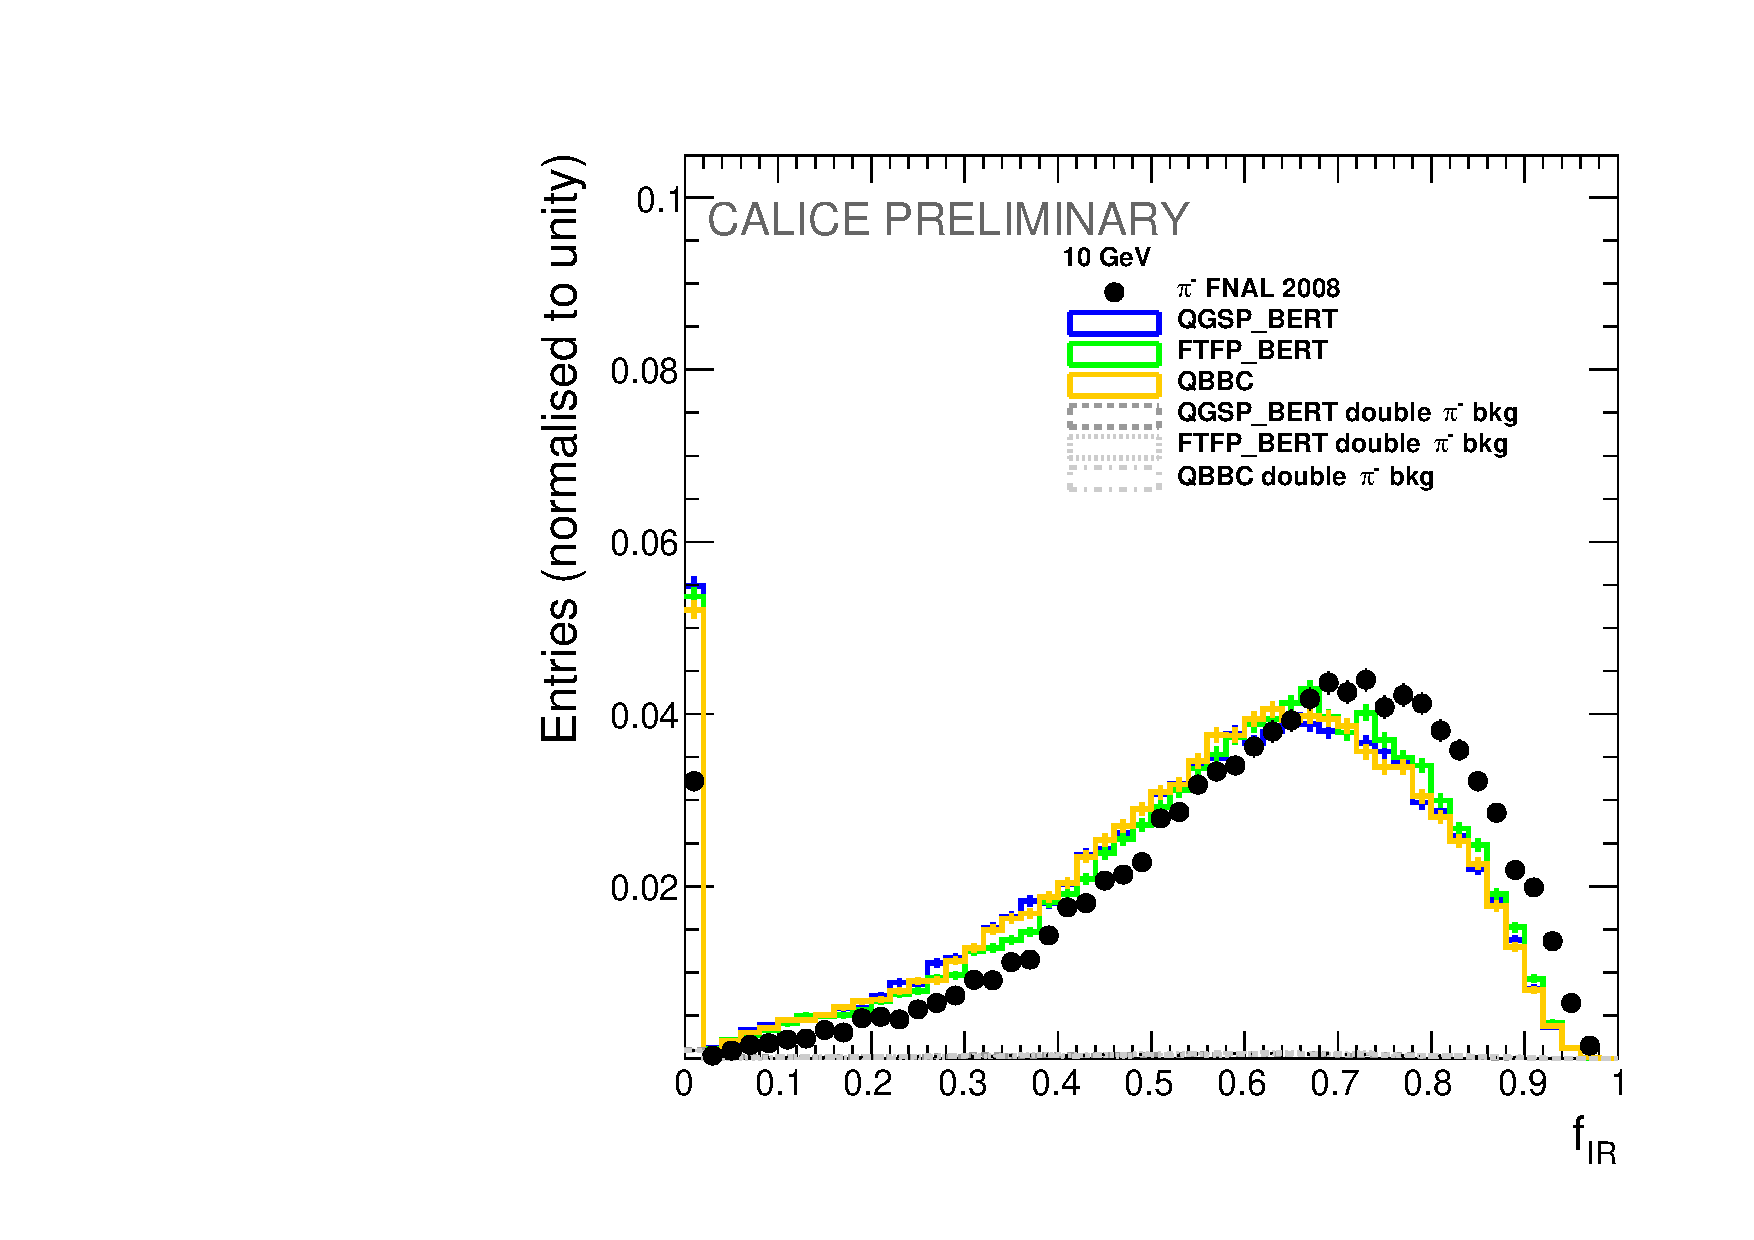
\includegraphics[width=.90\linewidth]{ECAL/plots/e-ir-10.pdf}
		\caption{\label{fig:efr10F} }
	\end{subfigure}
	\caption{\label{fig:irexampleF} \sl% {\bf Fig.~\ref{fig:efr2}: Remind me how the linear plot looks like} 
		Comparaison de $f_{IR}$ entre les données et les simulations pour trois {\sc Geant}4  listes physiques de l'\'energies 2 (a) et 10 (b) GeV de particule primordiale.}
\end{figure}

\begin{figure}
	\centering
	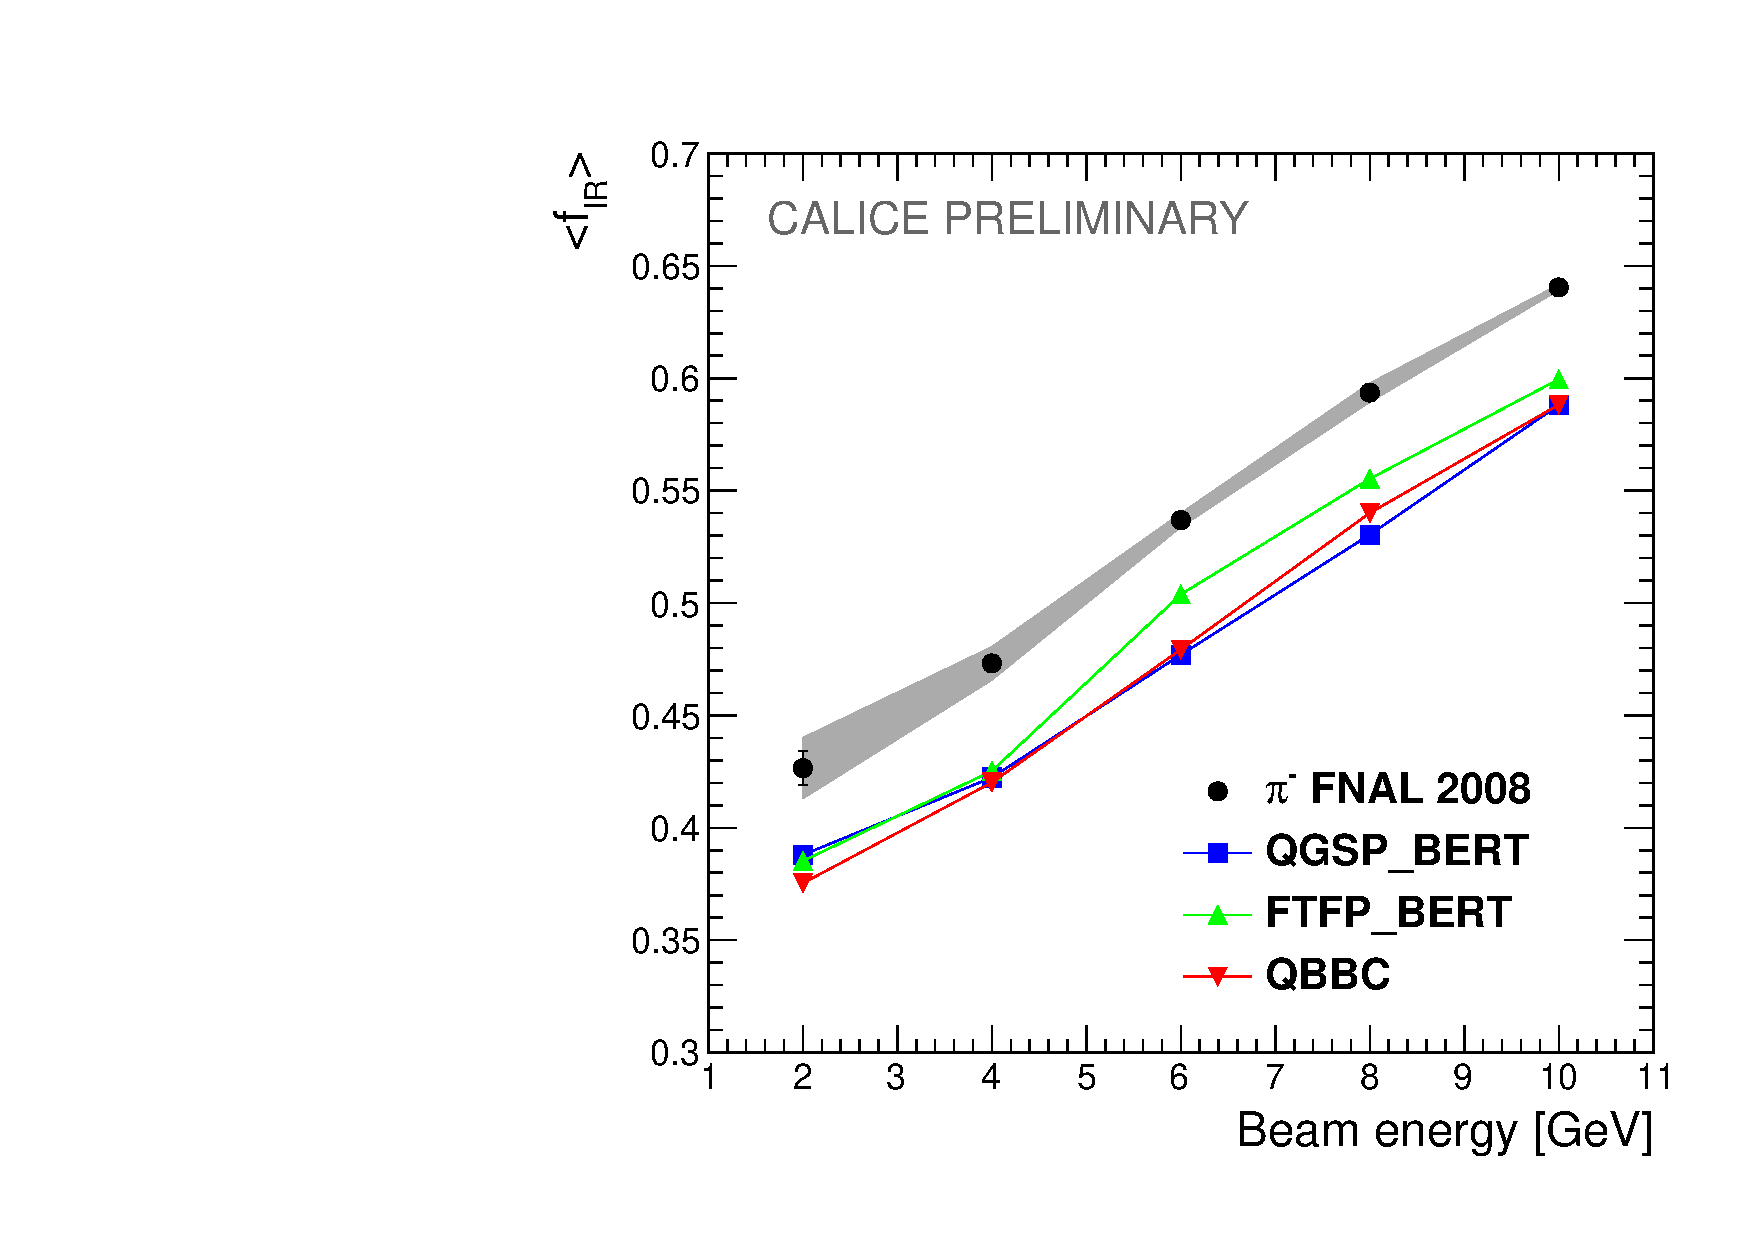
\includegraphics[width=0.5\textwidth]{ECAL/plots/e-ir-graph.pdf}
	\caption{\label{fig:irgraphF} \sl  Fraction moyenne du dépôt d'énergie dans la région d'interaction pour les données et les simulations  pour trois listes physiques \geant\ comme une fonction de l'énergie du faisceau (2 \, GeV à 10 \, GeV).}
\end{figure}

\begin{figure}
	\centering
	\begin{subfigure}{0.5\textwidth}
		\centering
		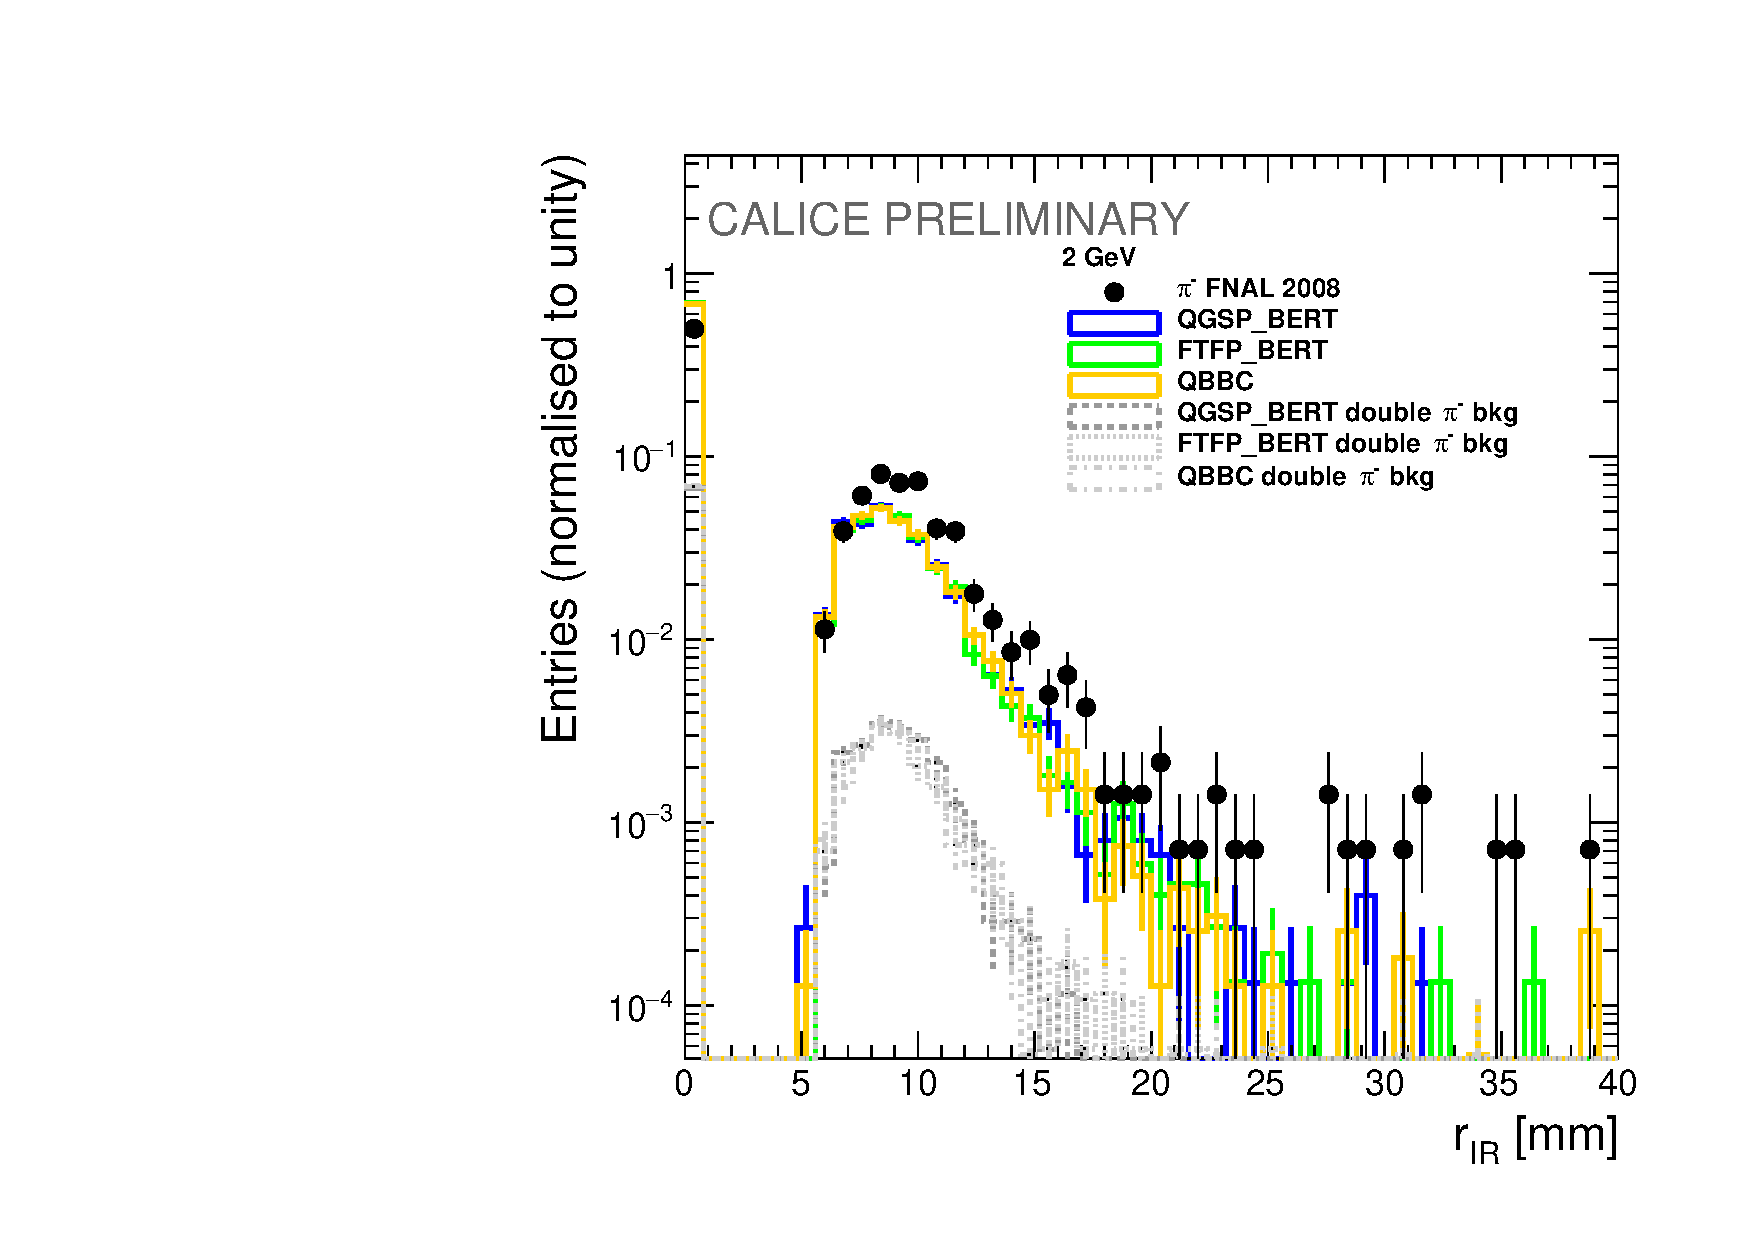
\includegraphics[width=.90\linewidth]{ECAL/plots/r-ir-2.pdf}
		\caption{\label{fig:rir2F} }
	\end{subfigure}% 
	\begin{subfigure}{0.5\textwidth}
		\centering
		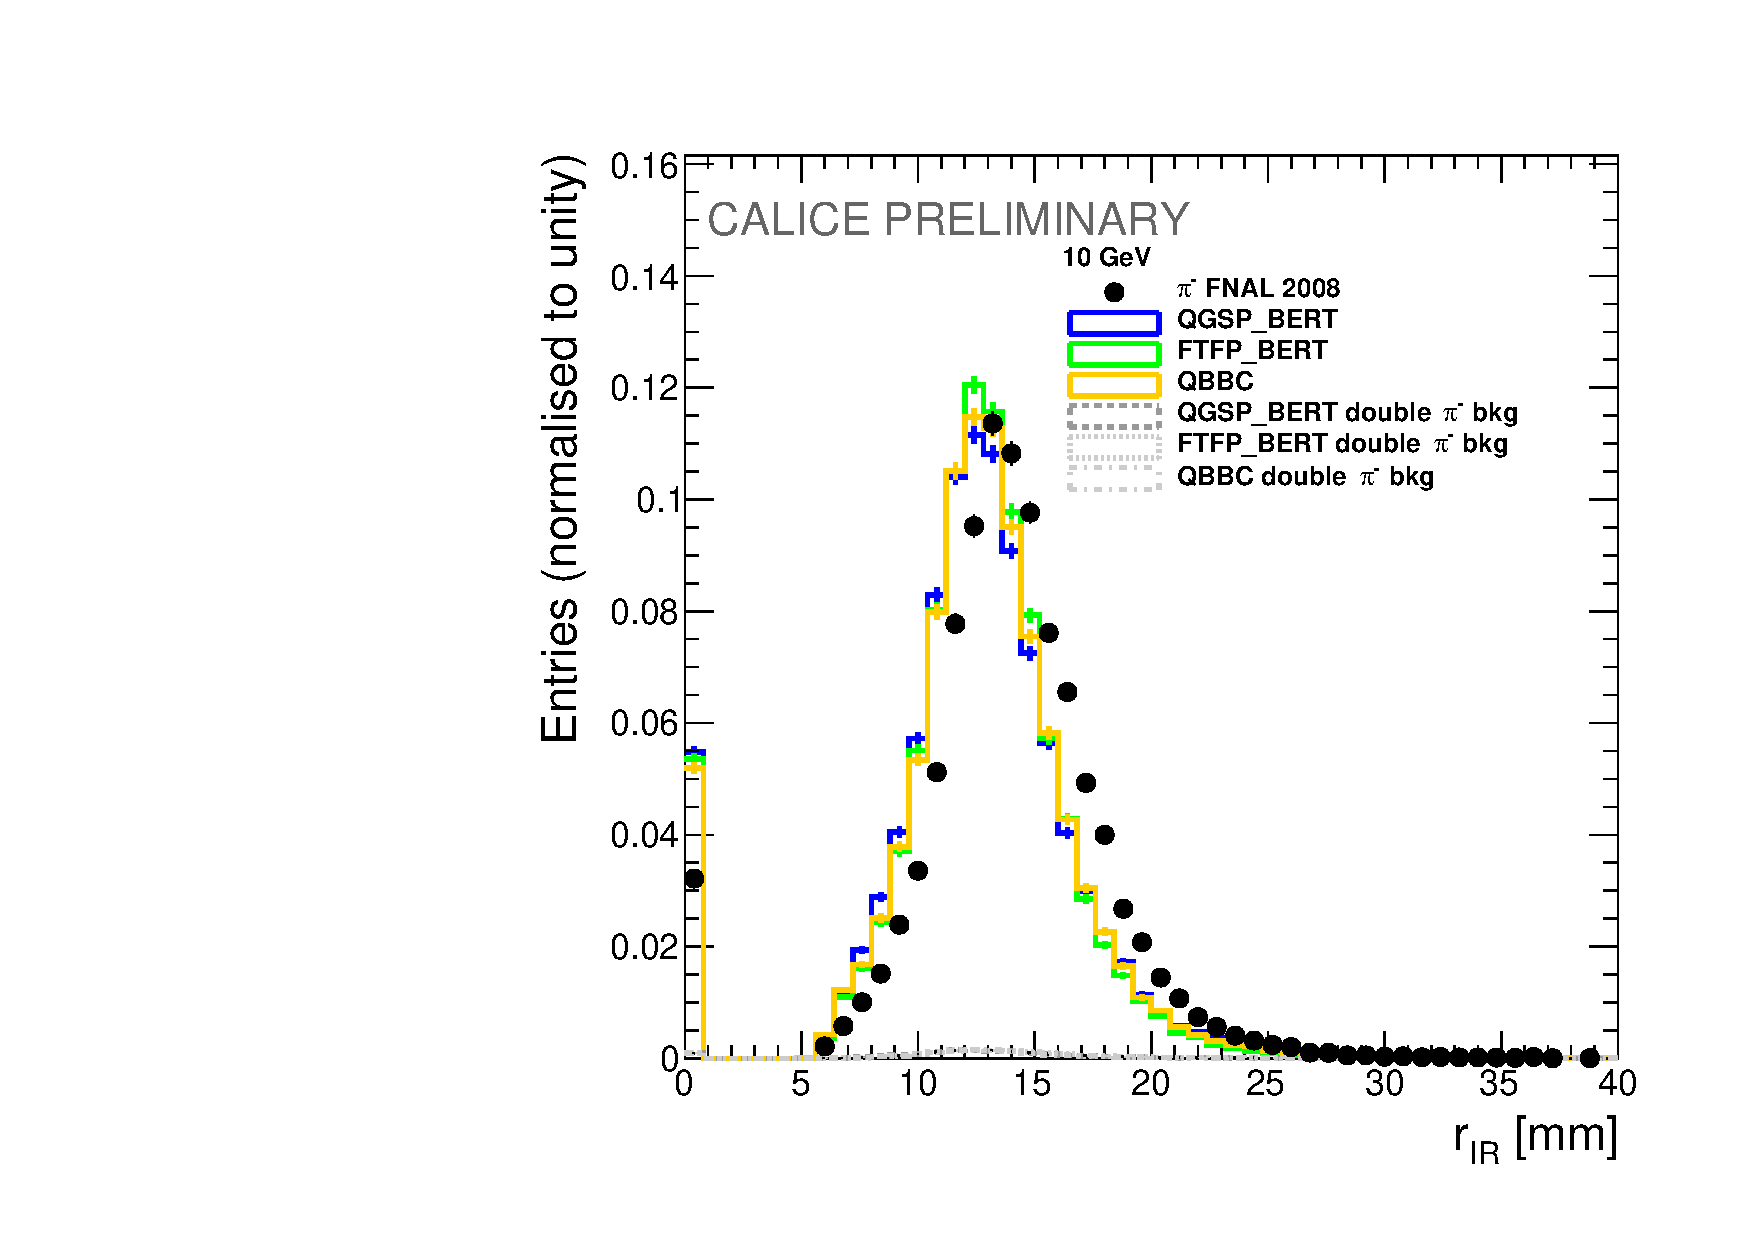
\includegraphics[width=.90\linewidth]{ECAL/plots/r-ir-10.pdf}
		\caption{\label{fig:rir10F} }
	\end{subfigure}
	\caption{\label{fig:rirexampleF} \sl %{\bf Same remark as for Fig.~\ref{fig:efr2} }
		Comparaison de $r_{IR}$ entre les données et les simulations pour trois {\sc Geant}4  listes physiques de l'\'energies 2 (a) et 10 (b) GeV de particule primordiale.}
\end{figure}

\begin{figure}
	\centering
	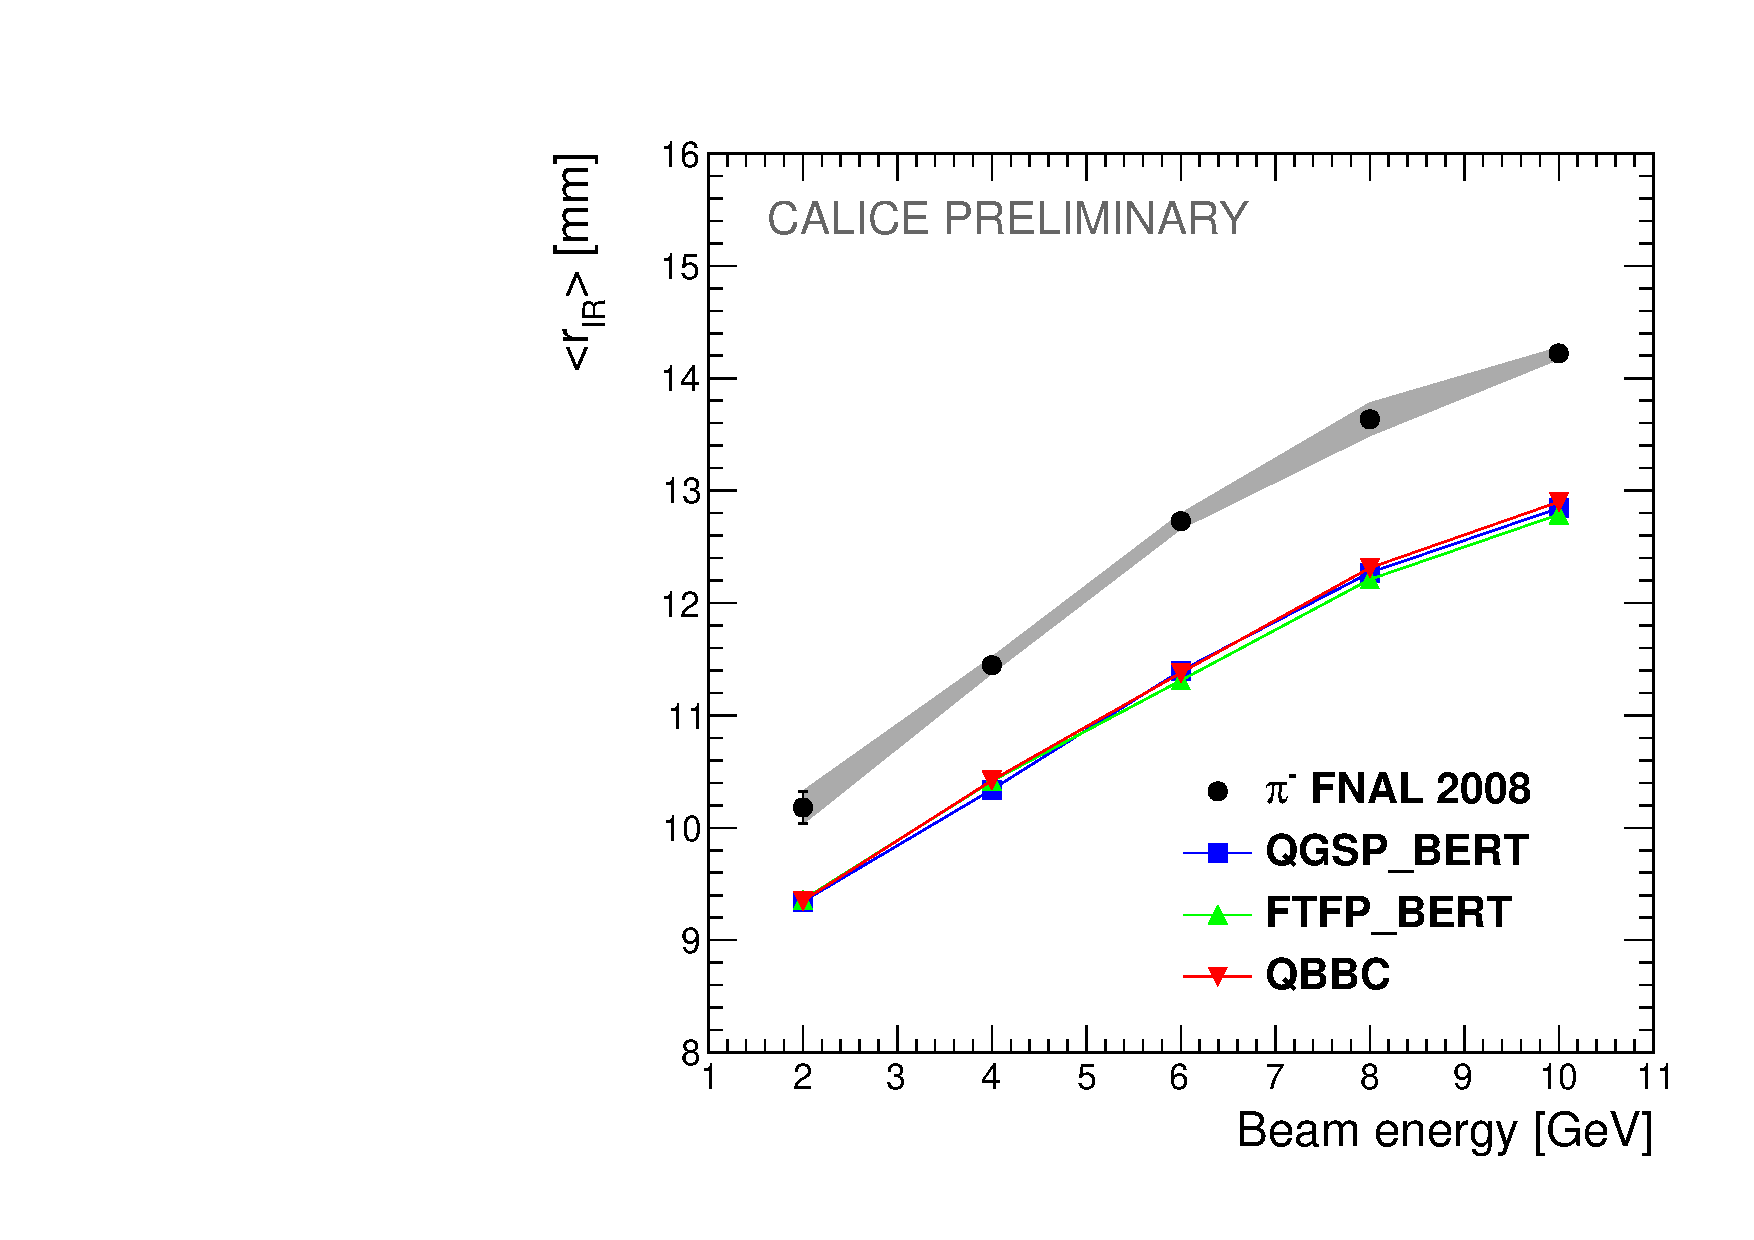
\includegraphics[width=0.5\textwidth]{ECAL/plots/r-ir-graph.pdf}
	\caption{\label{fig:irrgraphF} \sl Radius lateral moyen de la région d'interaction pour les données et les simulations  pour trois listes physiques \geant\ comme une fonction de l'énergie du faisceau (2 \, GeV à 10 \, GeV).}
\end{figure}

\begin{figure}
	\centering
	\begin{subfigure}{0.5\textwidth}
		\centering
		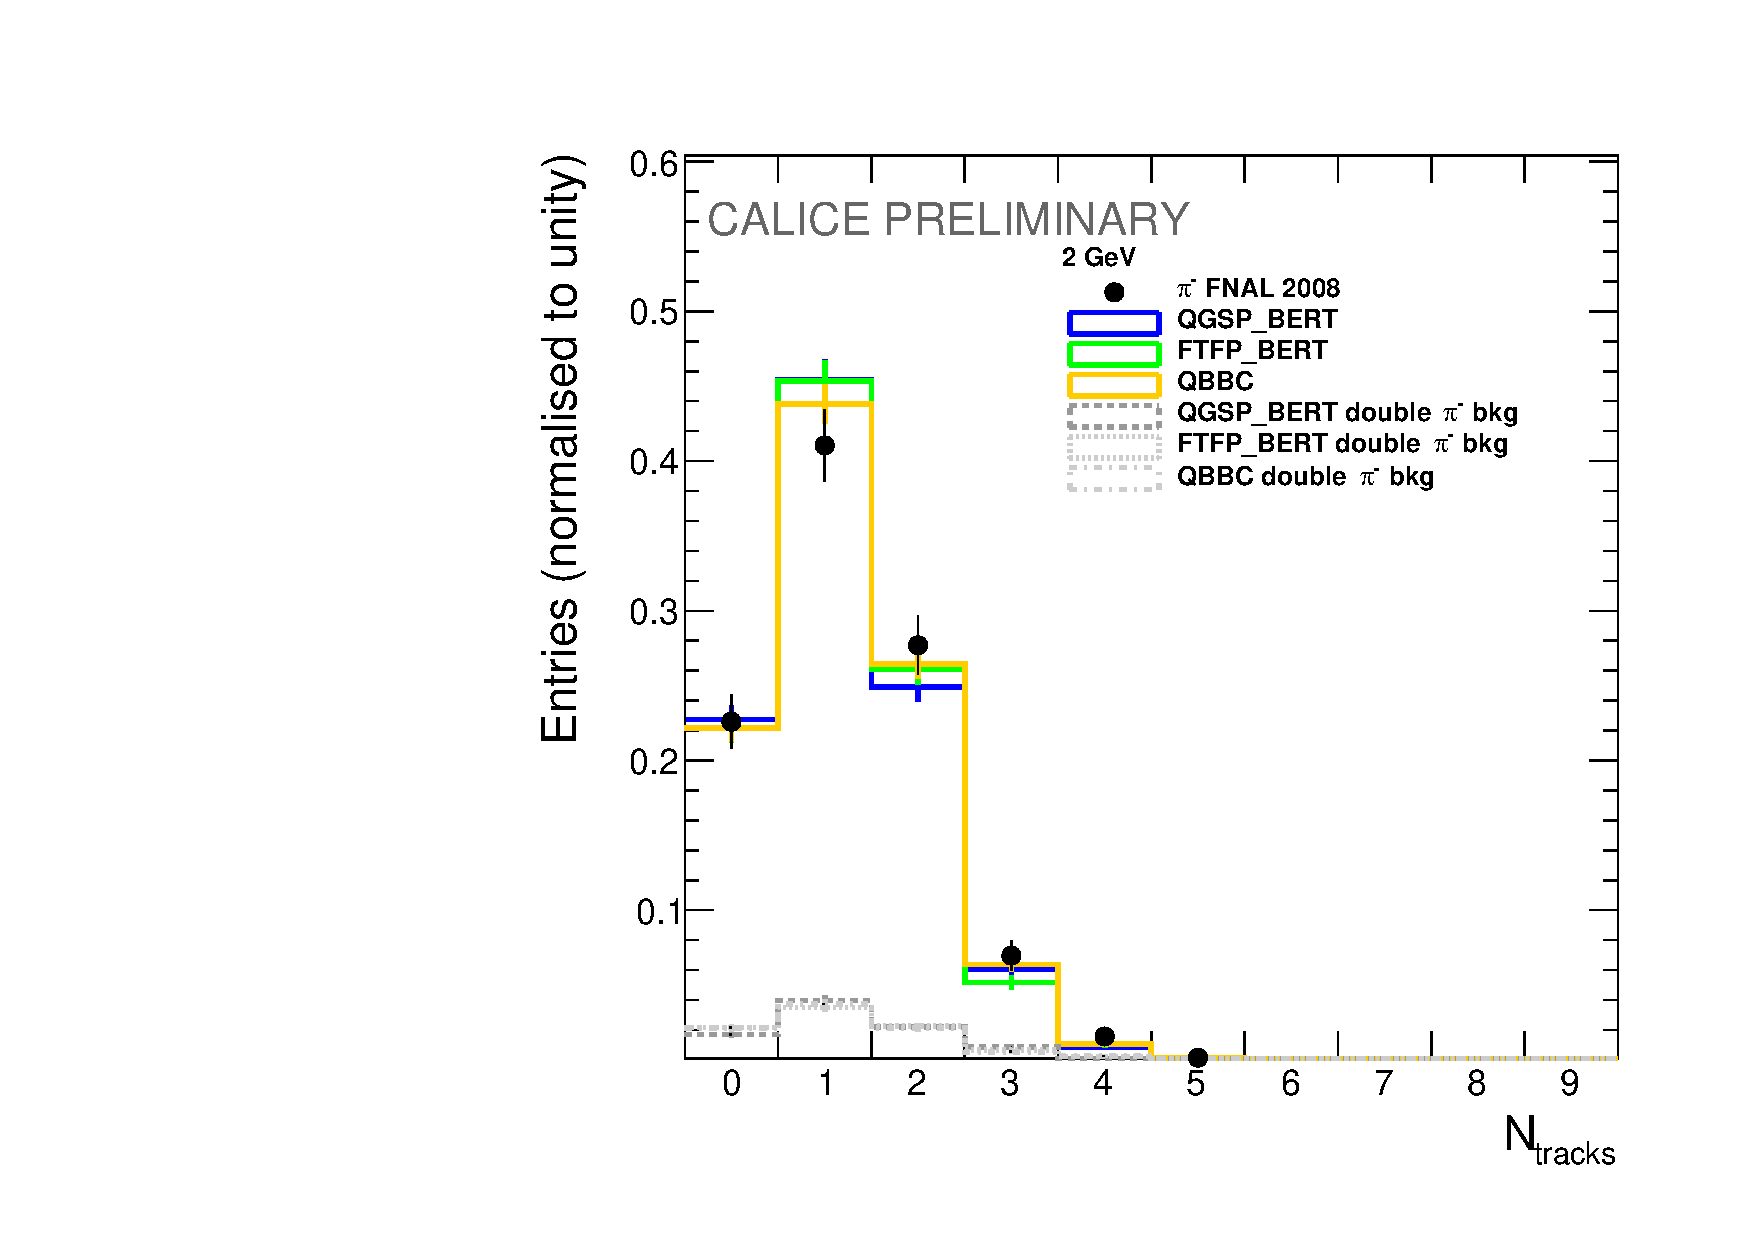
\includegraphics[width=.90\linewidth]{ECAL/plots/ntracks-2.pdf}
		\caption{\label{fig:tr2F} }
	\end{subfigure}% 
	\begin{subfigure}{0.5\textwidth}
		\centering
		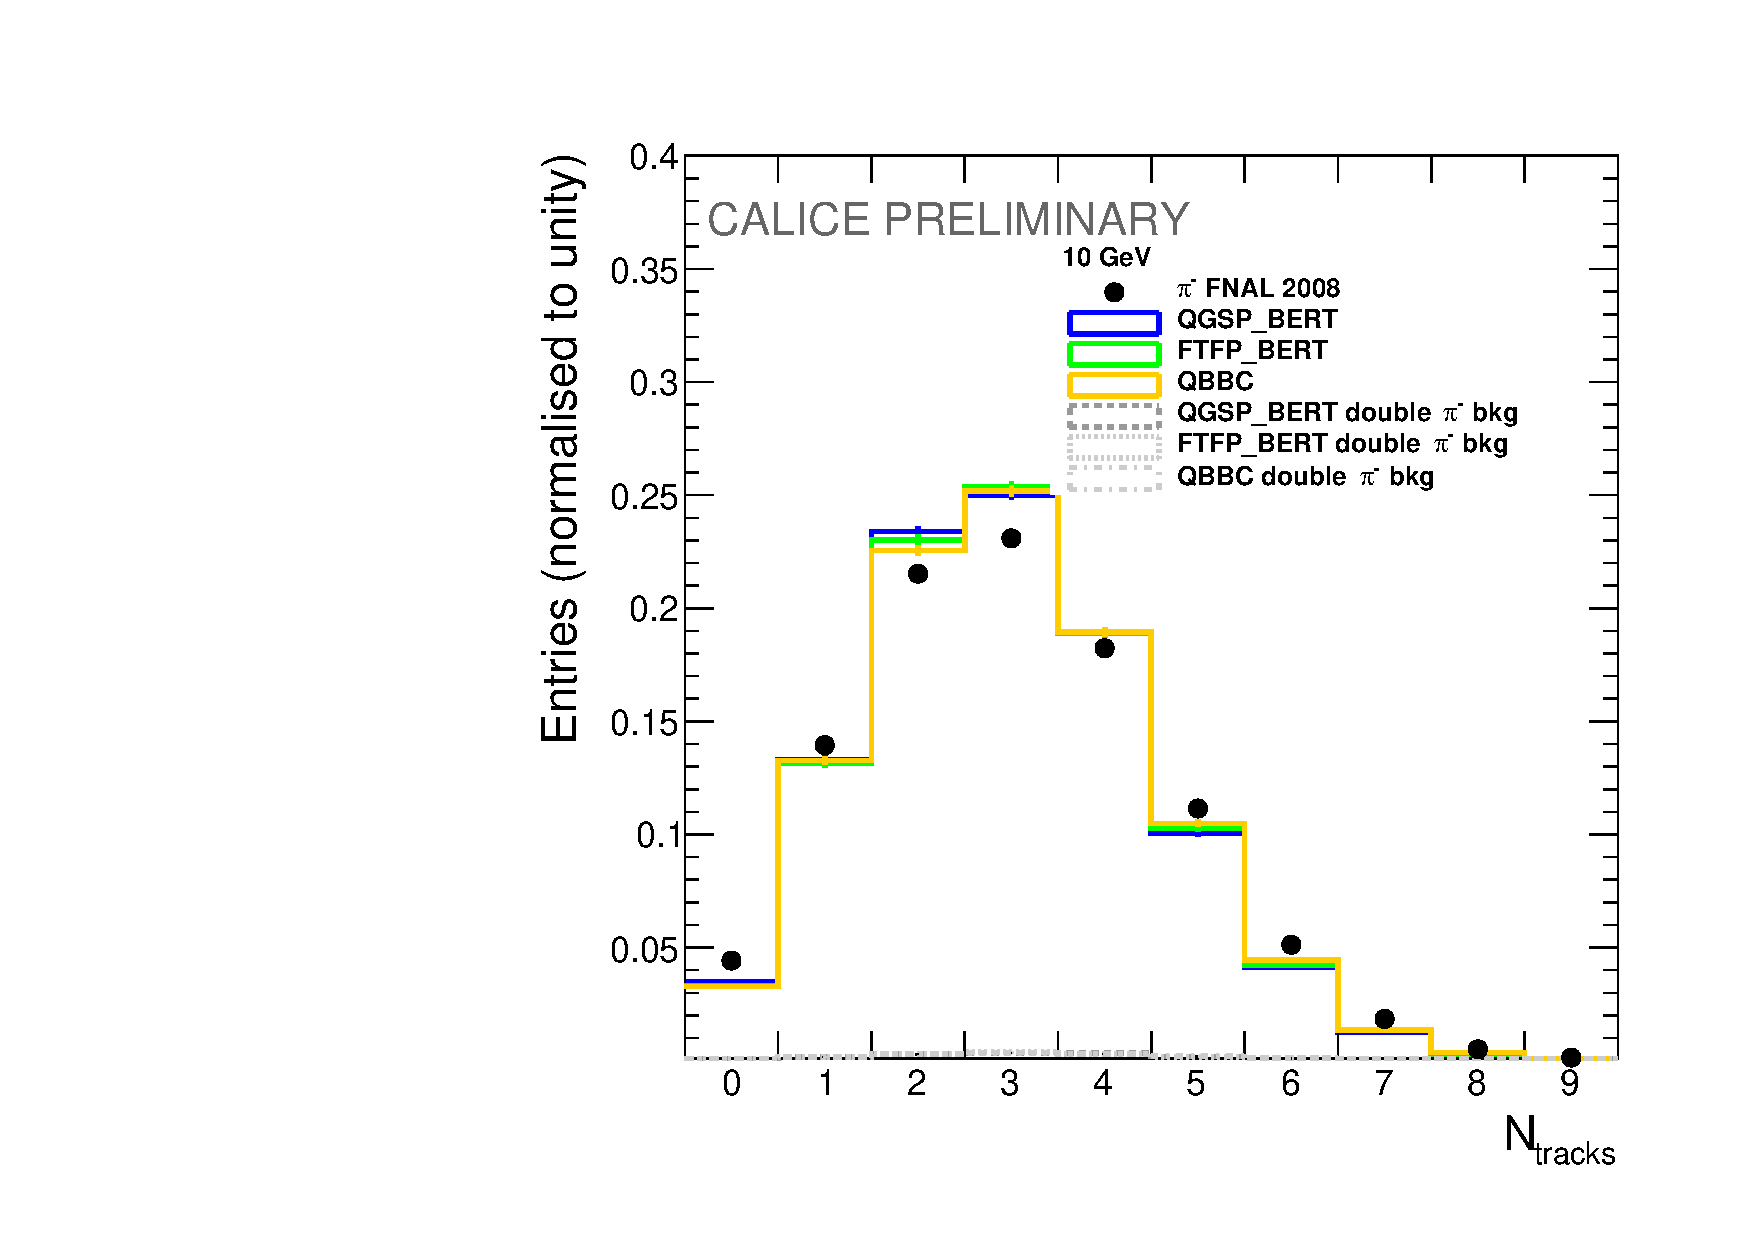
\includegraphics[width=.90\linewidth]{ECAL/plots/ntracks-10.pdf}
		\caption{\label{fig:tr10F} }
	\end{subfigure}
	\caption{\label{fig:trackexampleF} \sl Comparaison de $N_{tracks}$ entre les données et les simulations pour trois {\sc Geant}4  listes physiques de l'\'energies 2 (a) et 10 (b) GeV de particule primordiale.}
\end{figure}

\begin{figure}
	\centering
	\begin{subfigure}{0.5\textwidth}
		\centering
		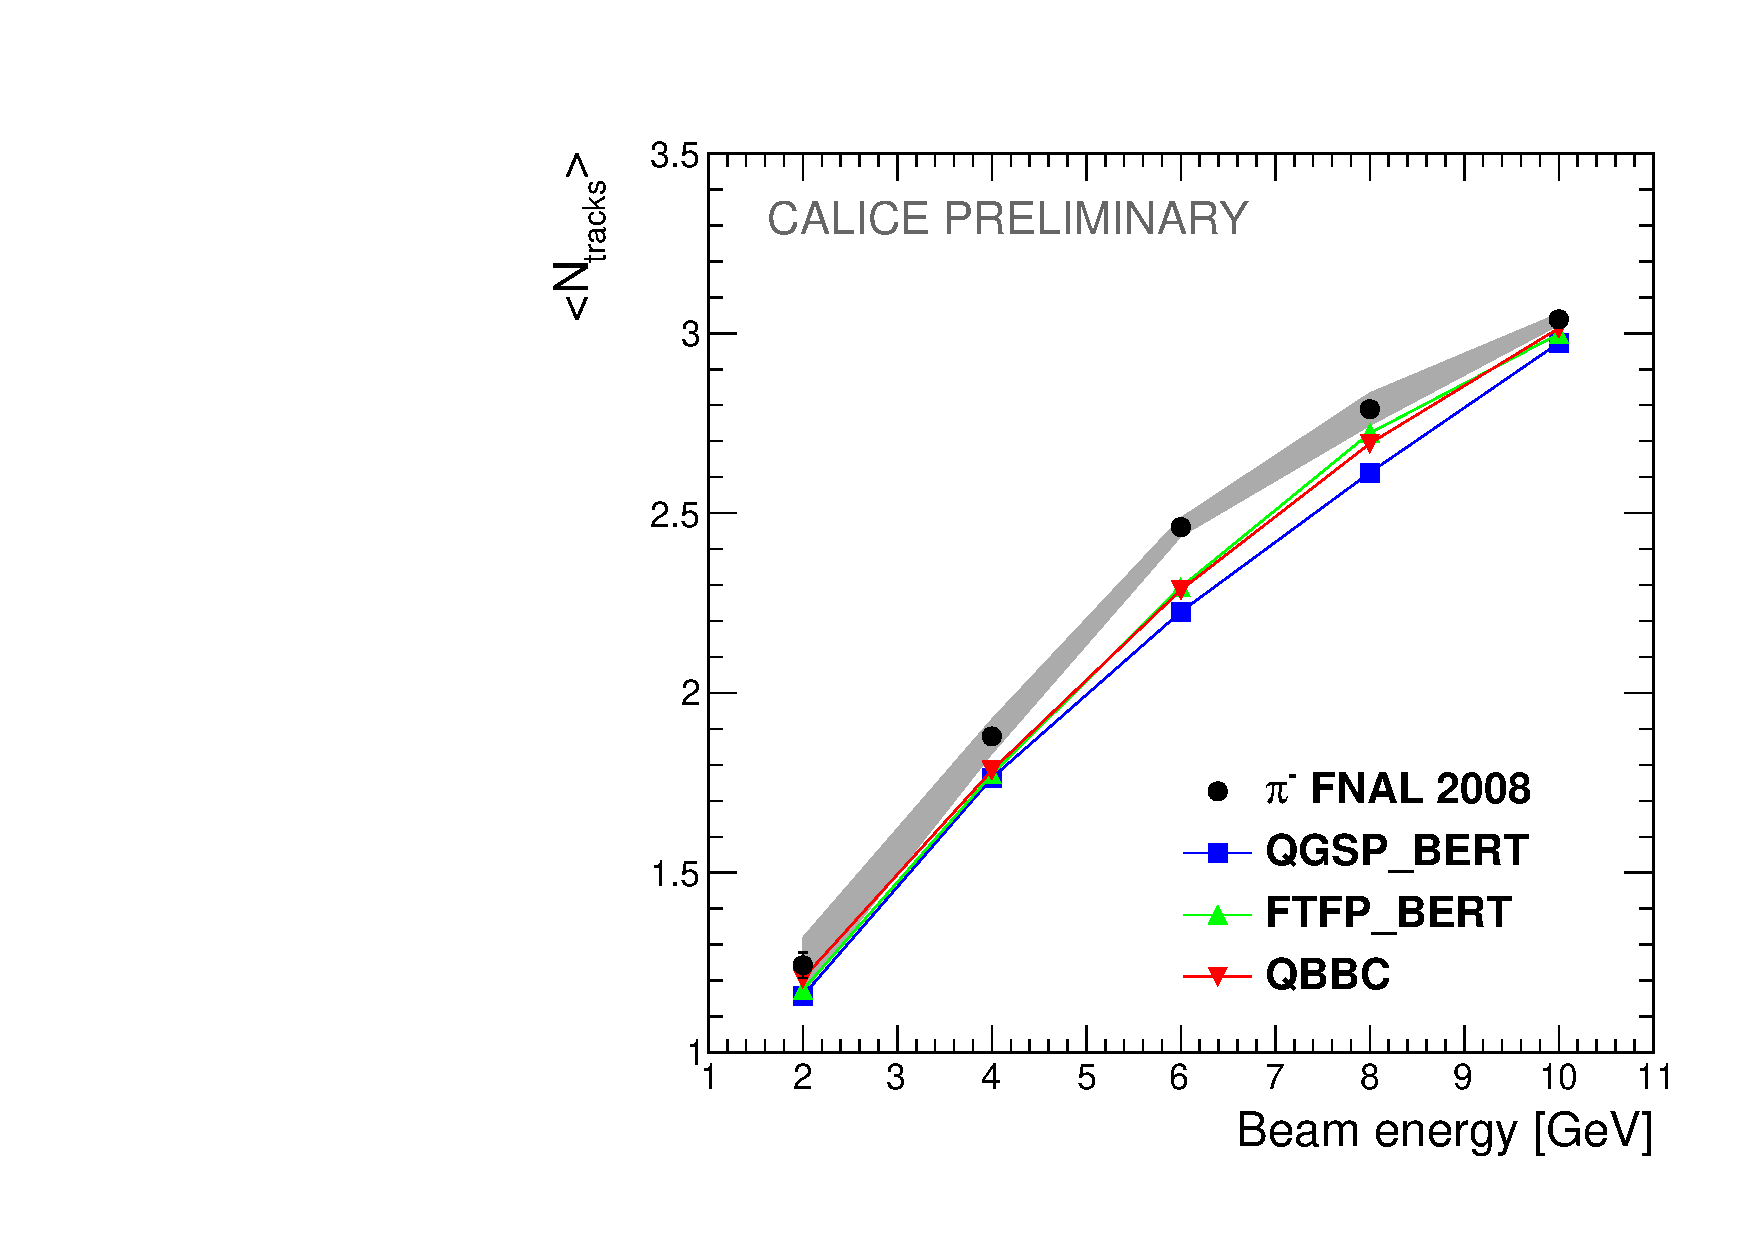
\includegraphics[width=.90\linewidth]{ECAL/plots/ntracks-graph.pdf}
		\caption{\label{fig:tracksgraphF} }
	\end{subfigure}% 
	\begin{subfigure}{0.5\textwidth}
		\centering
		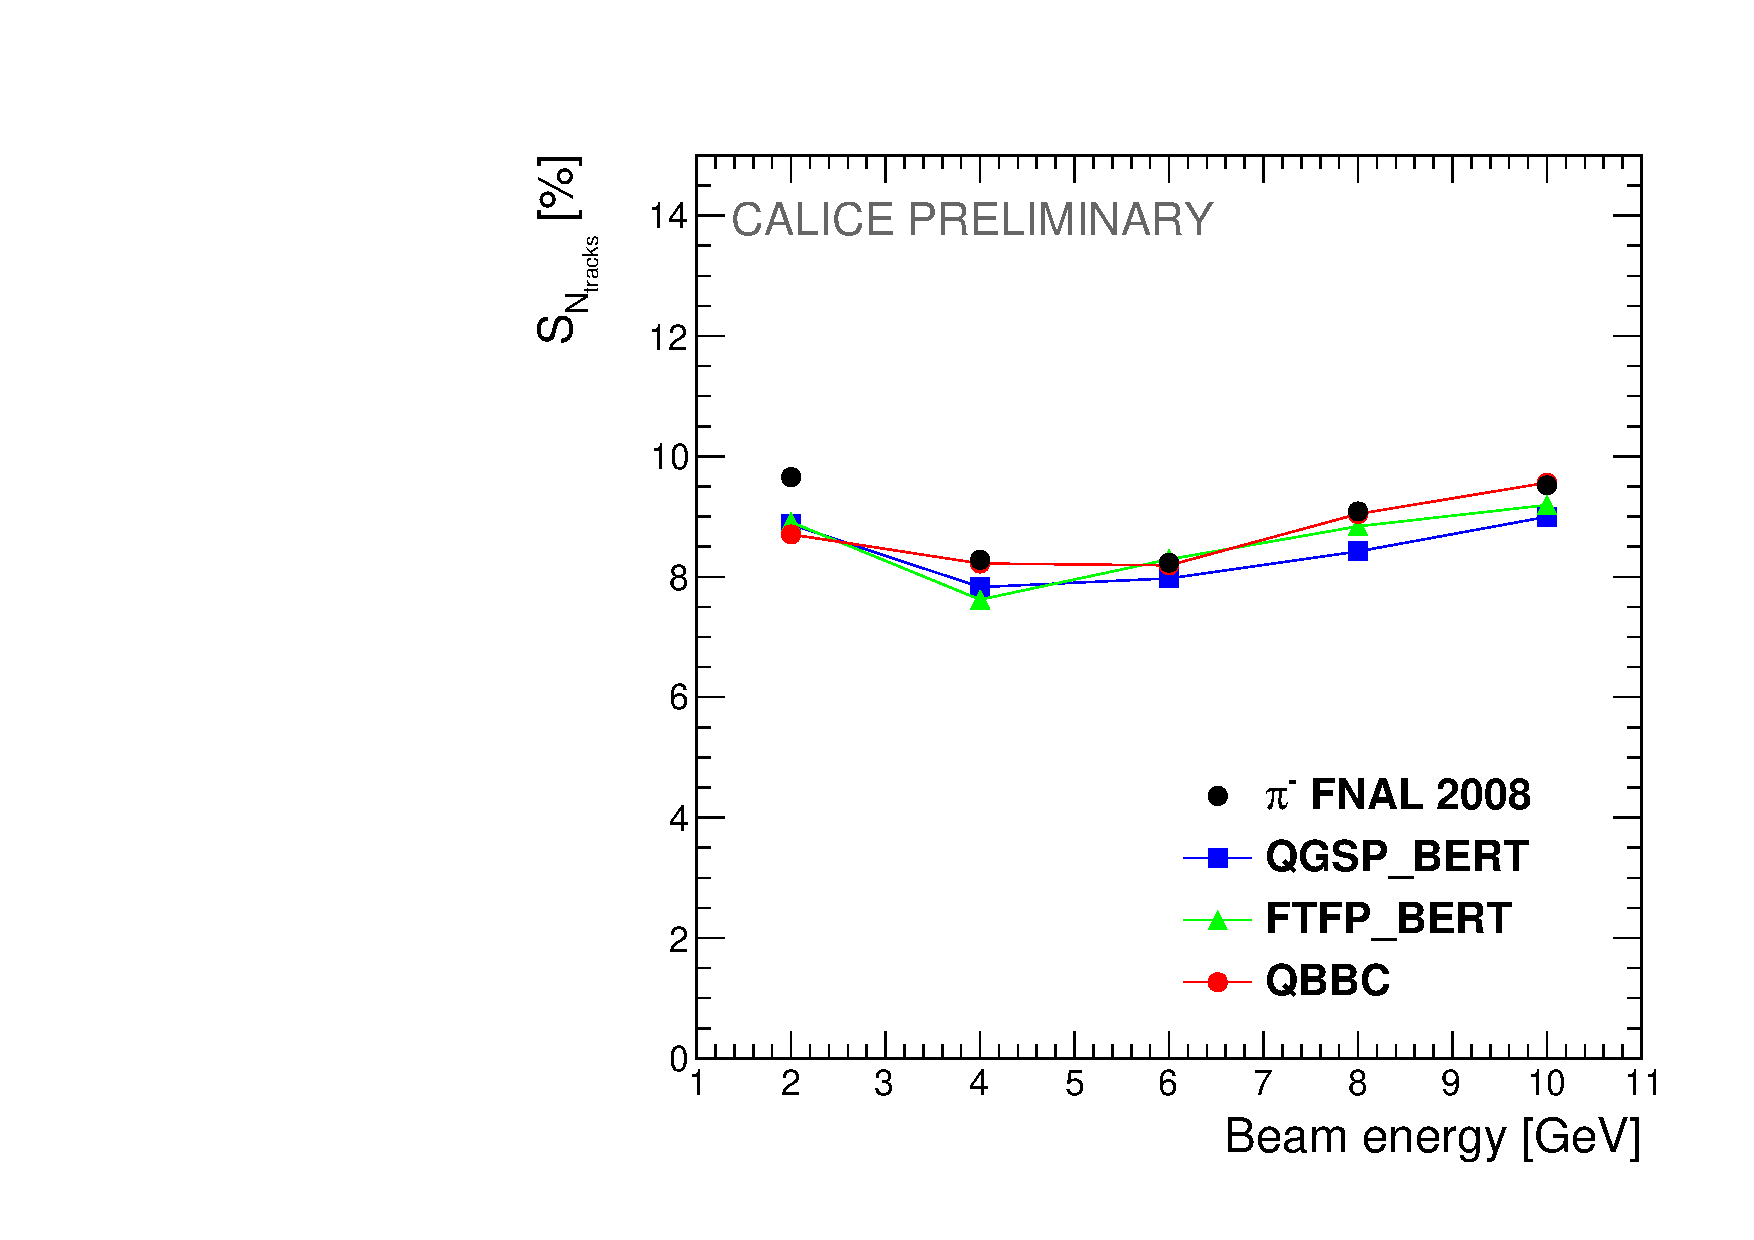
\includegraphics[width=.90\linewidth]{ECAL/plots/ntracks-graph-delta.pdf}
		\caption{\label{fig:dtracksgraphF}}
	\end{subfigure}
	\caption{\label{fig:fulltrackgraphF} \sl Moyenne du nombre des traces trouvées pour les données et les simulations  pour trois listes physiques \geant\ comme une fonction de l'énergie du faisceau (2 \, GeV à 10 \, GeV). }
\end{figure}


%-----------------------------------------------------------------------------
%-----------------------------------------------------------------------------
%-----------------------------------------------------------------------------

\subsection*{Les quarks top et bottom \'a l'ILC}
La production electrofaible des paires de fermions se déroule à travers le $f\bar{f}X$ vertex, où $X$ représente des bosons vectoriels neutres, un photon ou $Z^0$ boson. Le courant au $f\bar{f}X$ vertex peut être exprimé via les facteurs de forme $F$ comme:
\begin{equation}
\Gamma^{f\bar{f}X}_\mu (k^2,q,\bar{q}) = ie\{ \gamma_\mu (F^X_{1V}(k^2) + \gamma^5 F^X_{1A}(k^2)) - \frac{\sigma_{\mu\nu}(q-\bar{q})^\nu}{2m_f}(iF^X_{2V}(k^2) + \gamma^5 F^X_{2A}(k^2)) \},
\end{equation}
où $k^2= (q+\bar{q})^2$ st le quatri-moment au carré du boson du vecteur échangé, $q$ et $\bar{q} $ sont les quatri-momentes du fermion $f$ et antifermion $\bar{f}$ et $m_f$ est la masse fermion. Les $\gamma_\mu$ et $\gamma_5$ sont les matrices de Dirac, et $\sigma_{\mu\nu} = i/2(\gamma_\mu\gamma_\nu - \gamma_\nu\gamma_\mu)$.

Les valeurs de \sm\ du facteurs de forme sont les suivantes:
\begin{equation}
F^{f\gamma}_{1V} = Q^{f}, \ F^{f\gamma}_{1A} = 0, \ F^{fZ}_{1V} = \frac{I^f - 2Q^f\sin^2\theta_W}{2\cos\theta_W\sin\theta_W}, \ F^{fZ}_{1A} = - \frac{I^f}{2\cos\theta_W\sin\theta_W},
\label{formula:SMformFactors_3F}
\end{equation}
et toutes les facteurs $F_2$ sont zéros. Dans l'equation~\ref{formula:SMformFactors_3F} $I^f$ est  l'isospin faible, $I^t = 1/2$ pour top et $I^b = -1/2$ pour quark bottom  et $Q^f$ est le charge electrique, $Q^t = 2/3$ et $Q^b = -1/3$.

%The form factors are related to fermion couplings with left and right-handed helicity to $Z^0$ boson:
La définition suivante des couplages gauches et droites $Z^0b\bar{b}$ est utilisée tout au long de la thèse: 
\begin{equation}
%g_L^Z = (F_{1V}^Z - F_{1A}^Z), \  g_R^Z = F_{1V}^Z + F_{1A}^Z, 
g_L^Z = I^f - Q^f\sin^2\theta_W, \  g_R^Z = -Q^f\sin^2\theta_W.
\label{formula:EWcouplings_3F}
\end{equation}

%-----------------------------------------------------------------------------
%-----------------------------------------------------------------------------
%-----------------------------------------------------------------------------

\subsection*{Reconstruction de la charge du quark bottom}

\begin{figure}
	{\centering
		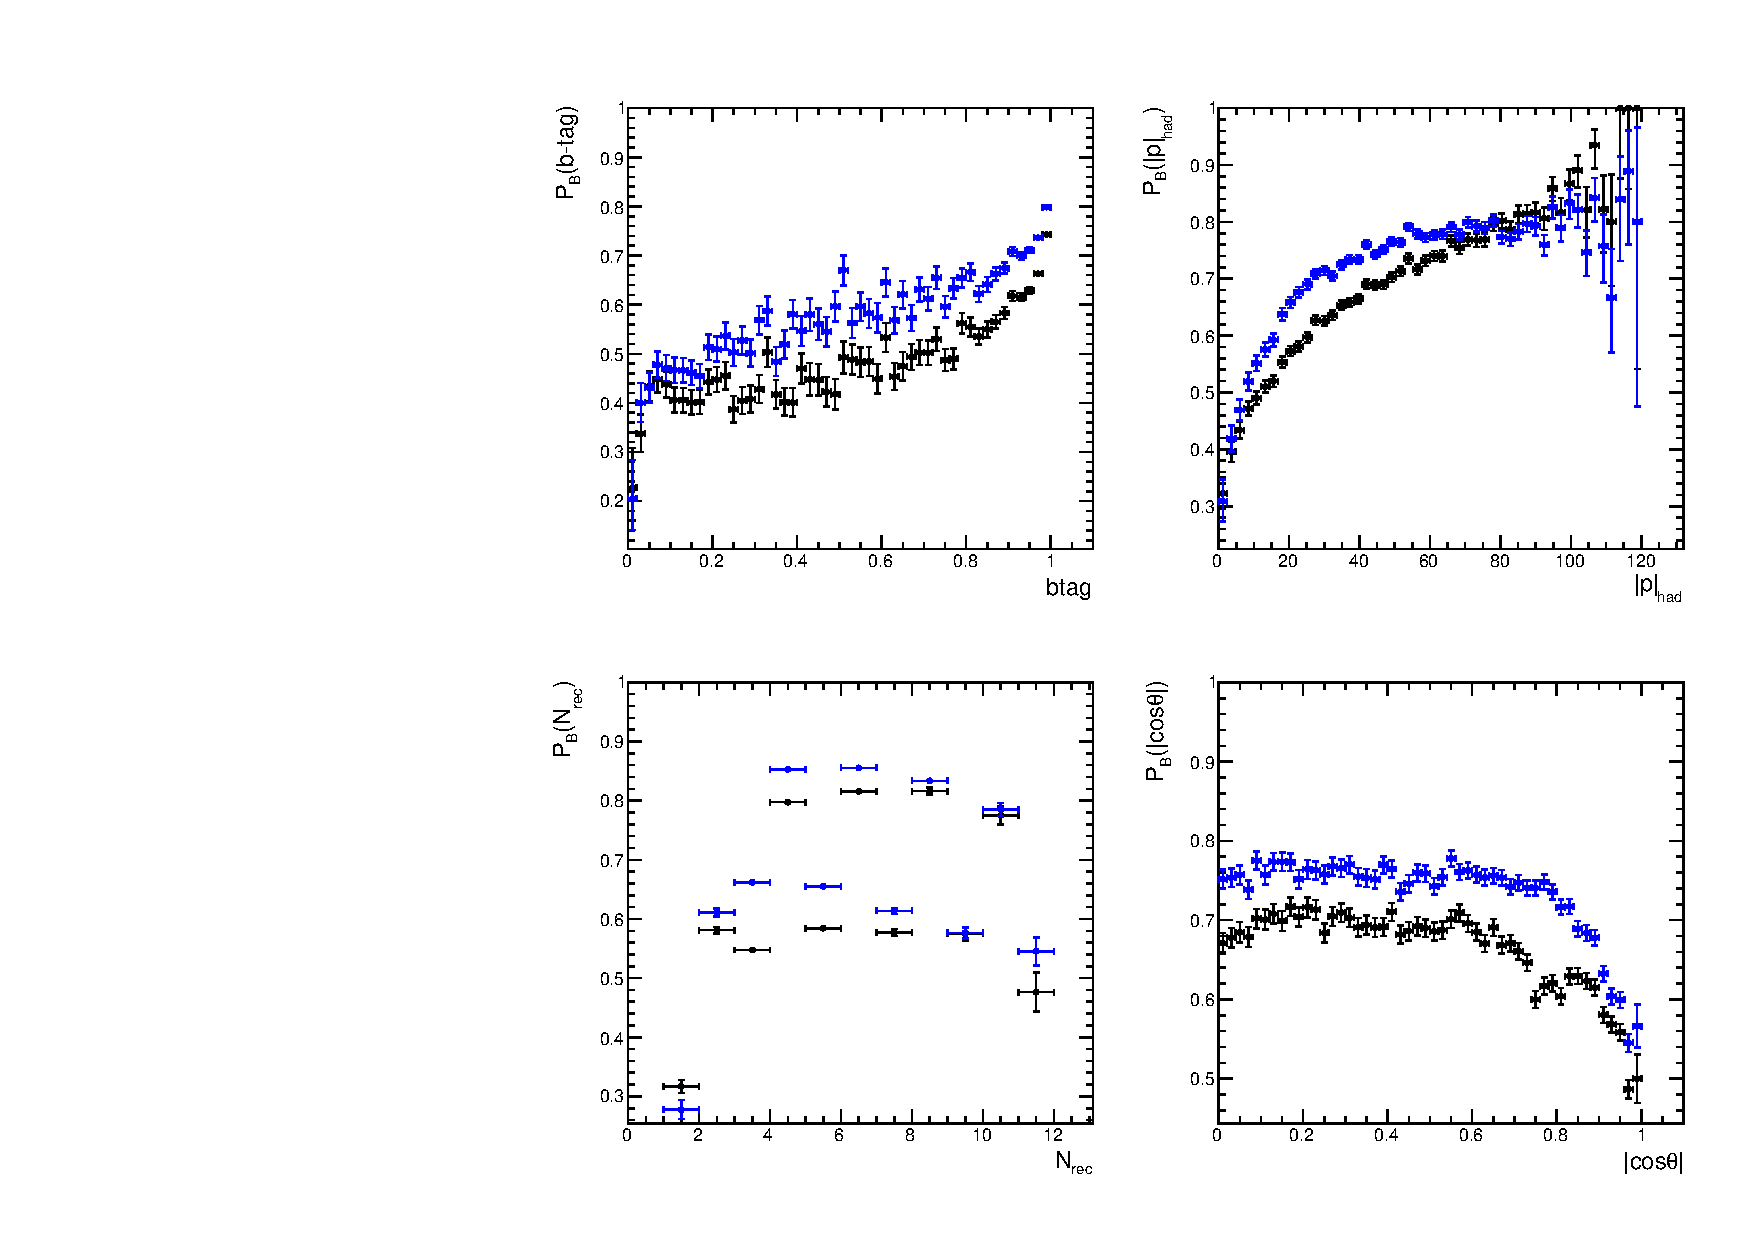
\includegraphics[width=0.95\textwidth]{ILD/plots/recovery-purity-comparison.pdf}
		\caption{\sl Comparaison de la pureté en fonction de b-tag, moment de b-hadron reconstruit, $N_ {rec}$ et l'angle polaire $|\cos\theta|$ avant et après l'algorithme de récupération de vertex. 
		}
		\label{fig:RecoveryPurityComparison_3F}
	}
\end{figure}

\begin{figure}
	{\centering
		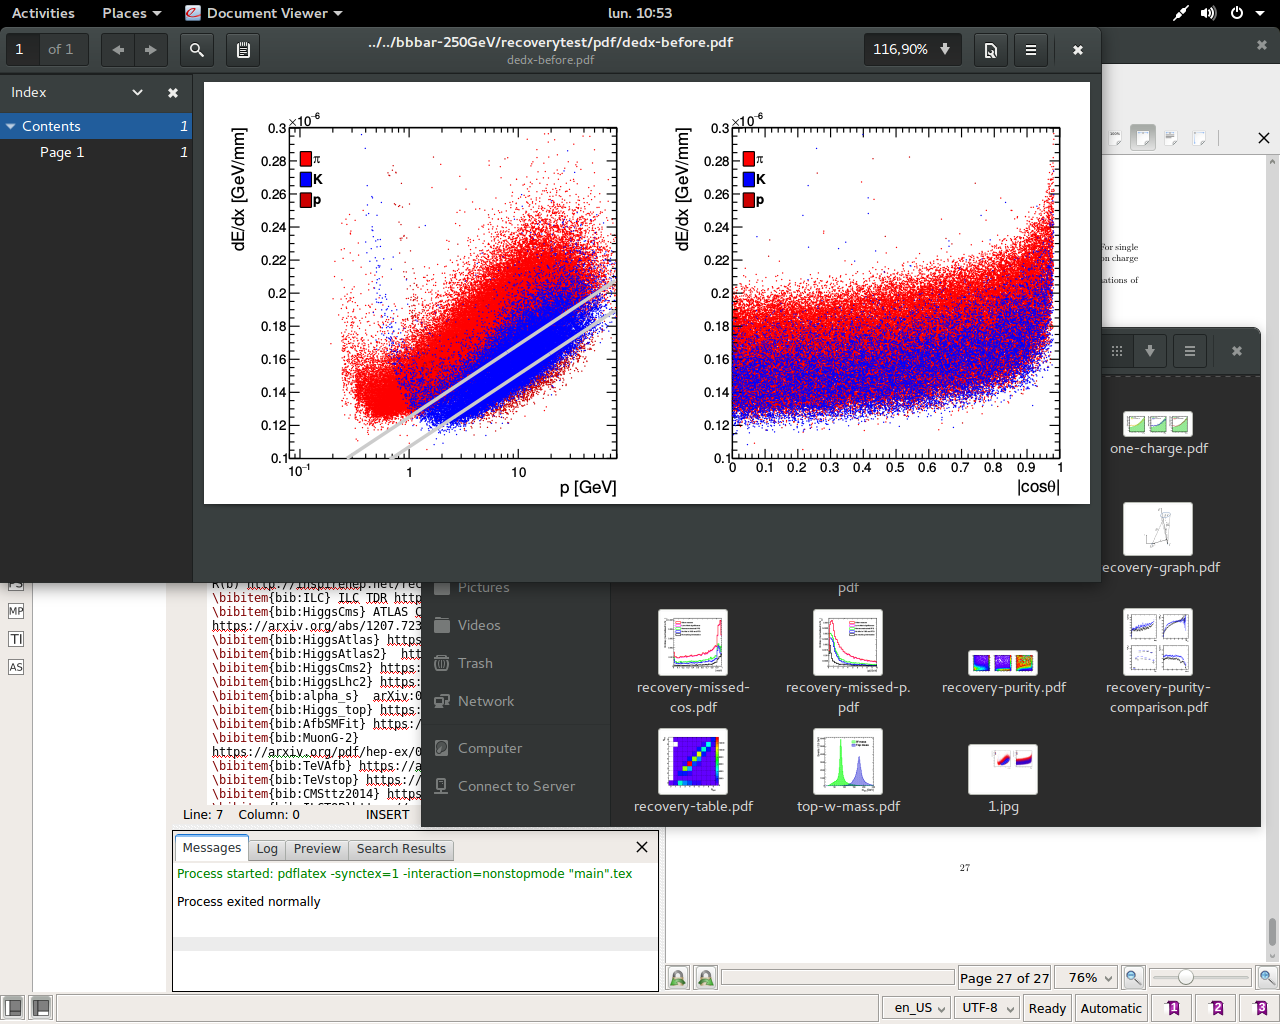
\includegraphics[clip, trim=8cm 18.5cm 7cm 4cm,width=0.95\textwidth]{ILD/plots/dedx-before.png}
		\caption{\sl Le dépôt d'énergie par longueur de trace $dE/dx$ en fonction de moment des particules, l'angle polaire des particules $|\cos\theta|$ pour différentes types des particules. Deux lignes grises séparent la région avec une concentration maximale de kaon.
		}
		\label{fig:dEdxBefore_3F}
	}
\end{figure}

\begin{figure}
	{\centering
		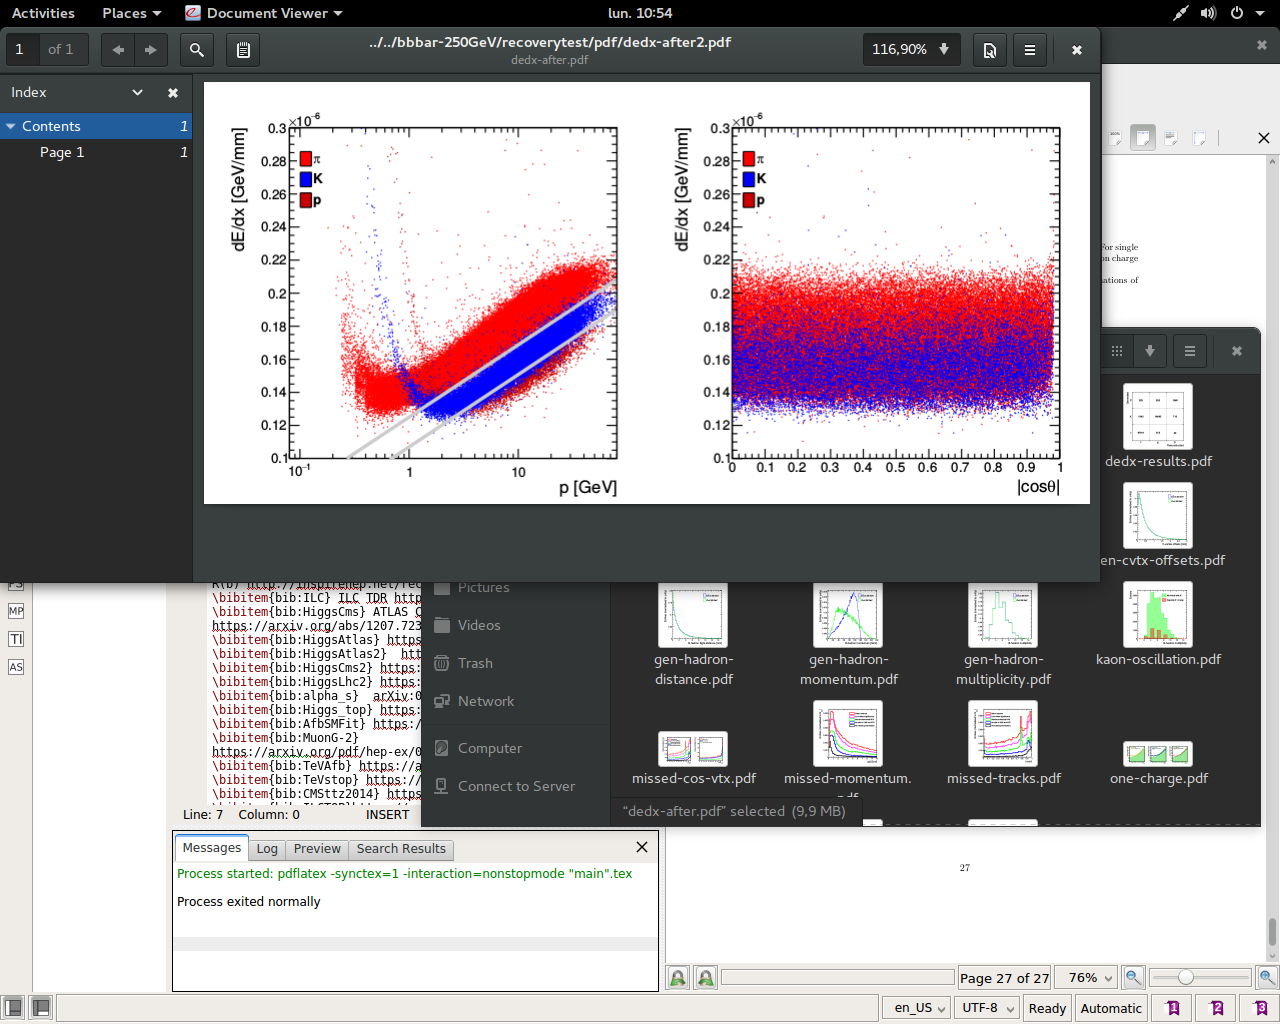
\includegraphics[clip, trim=8cm 18.5cm 7cm 4cm, width=0.95\textwidth]{ILD/plots/dedx-after.png}
		\caption{\sl Le dépôt d'énergie par longueur de trace $dE/dx$ en fonction de moment des particules, l'angle polaire des particules $|\cos\theta|$ pour différentes particules. apr\'es l'application de correction angulaire.  Deux lignes grises séparent la région avec une concentration maximale de kaon.
		}
		\label{fig:dEdxAfter_3F}
	}
\end{figure}


%-----------------------------------------------------------------------------
%-----------------------------------------------------------------------------
%-----------------------------------------------------------------------------

\subsection*{Reconstruction de l'angle polaire du quark top}


\begin{figure}
	\centering
	\begin{subfigure}{0.5\textwidth}
		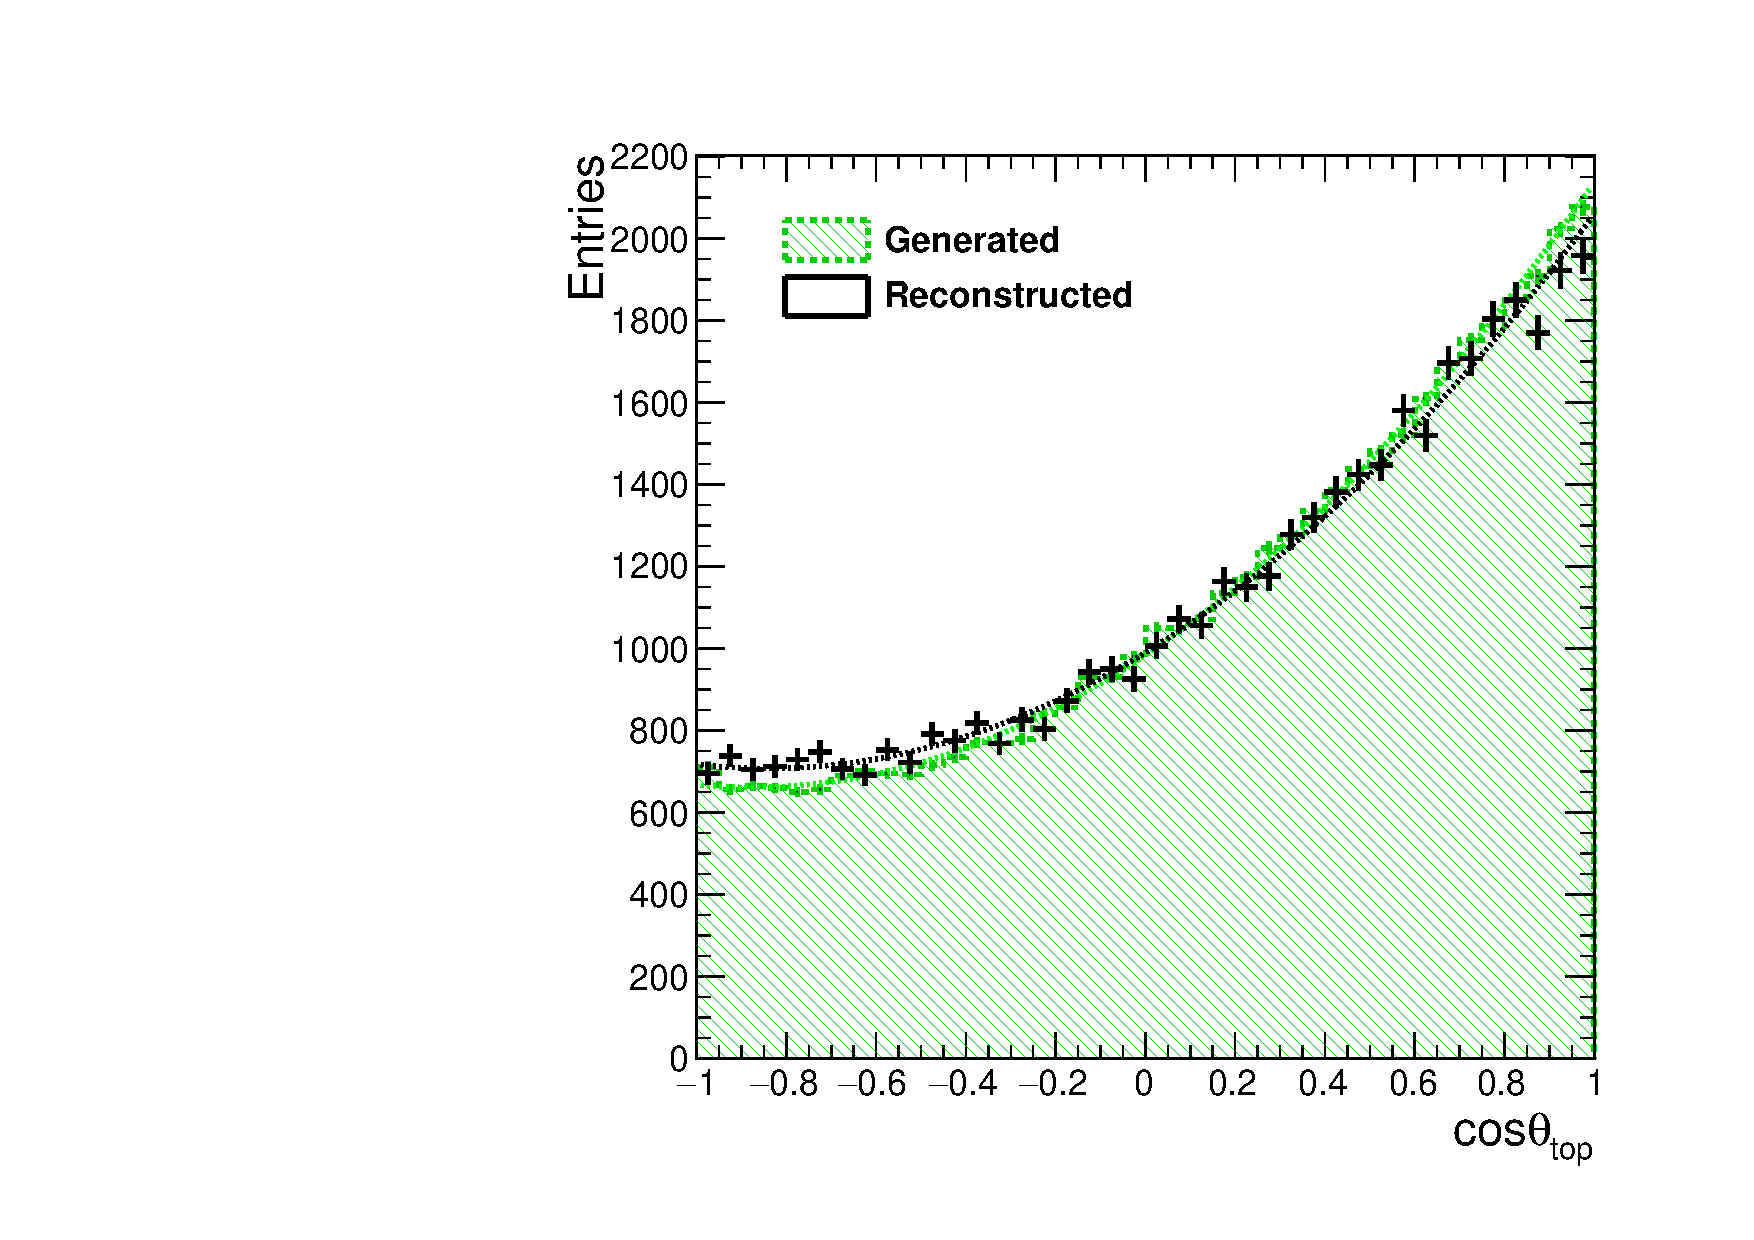
\includegraphics[width=0.95\textwidth]{ILD/plots/top-asymmetry-lepton.pdf}
		\caption{\label{fig:TopAsymmetryChi_a_3F} }
	\end{subfigure}% 
	\begin{subfigure}{0.5\textwidth}
		\centering
		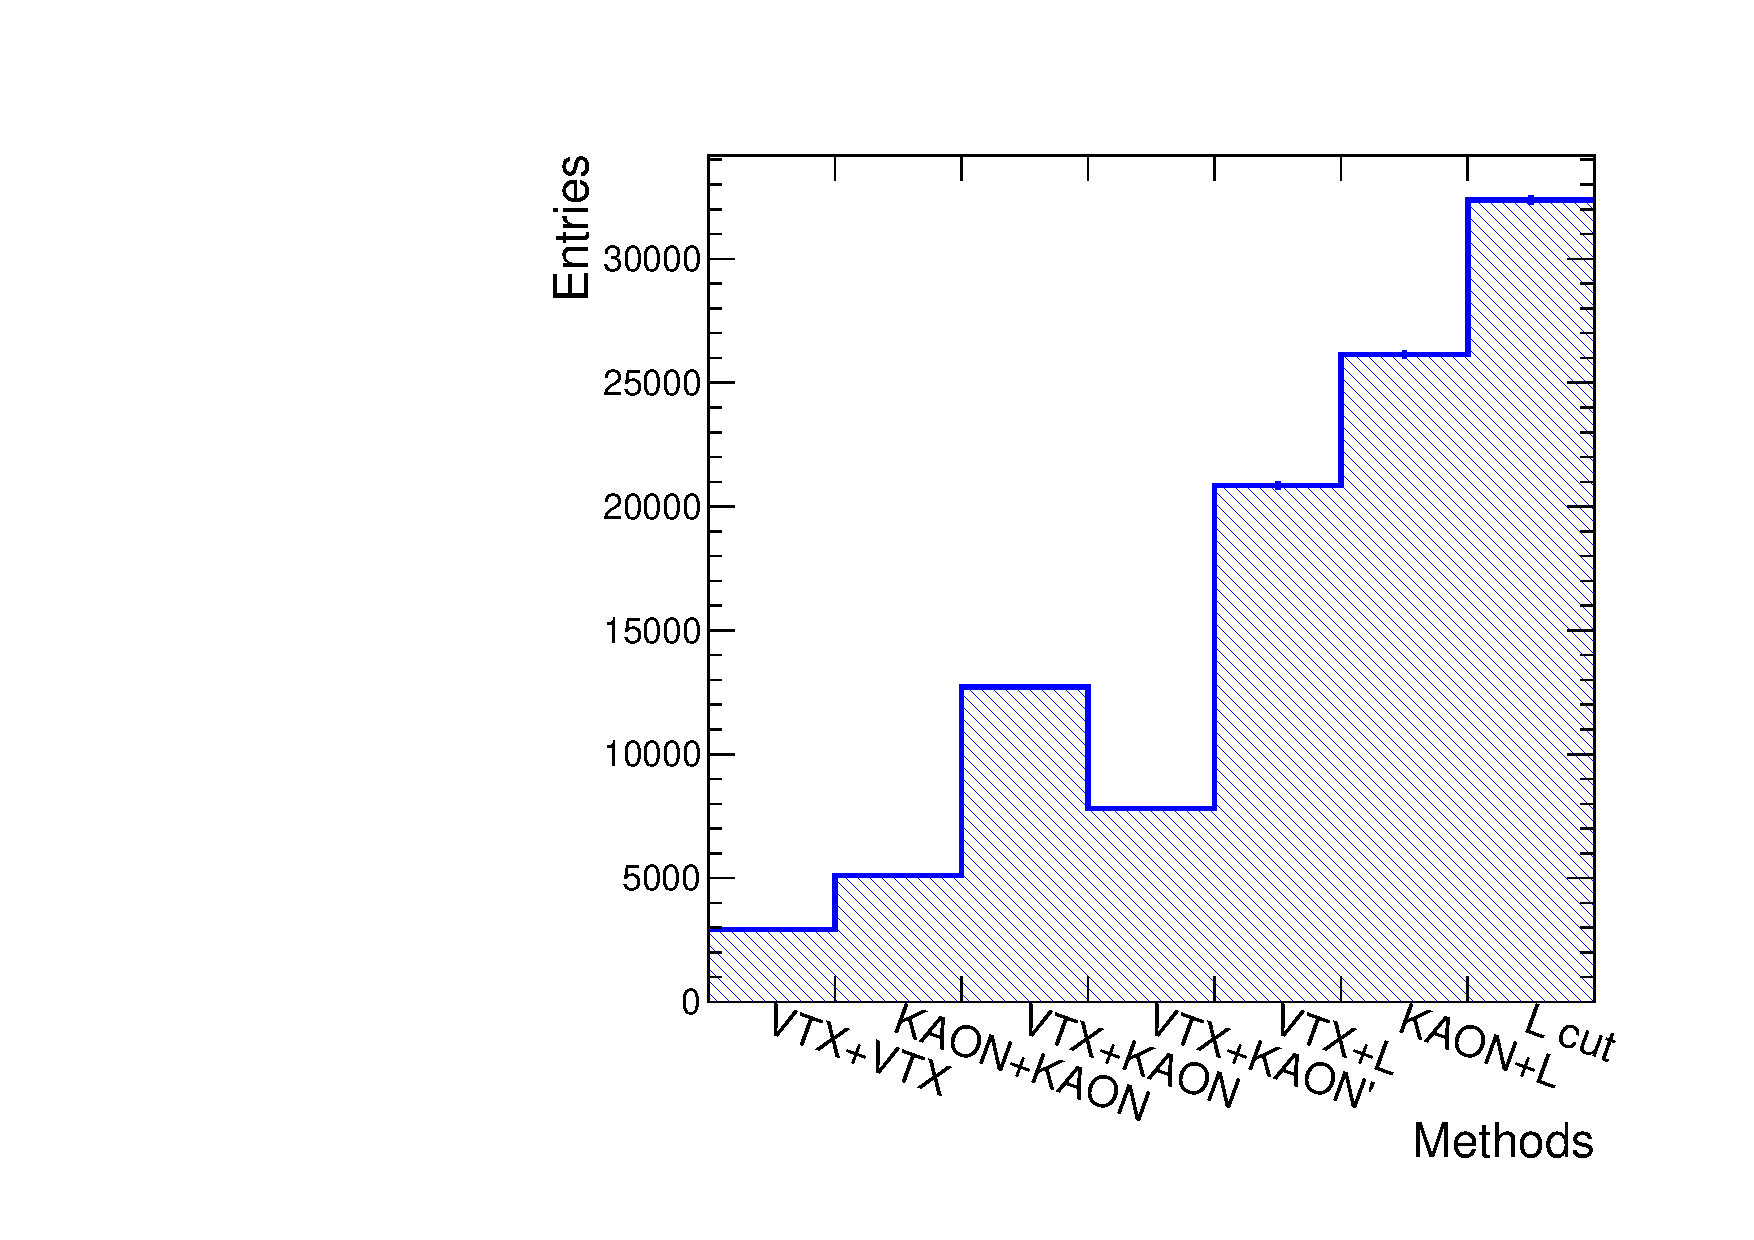
\includegraphics[width=0.95\textwidth]{ILD/plots/top-methods-lepton.pdf}
		\caption{\label{fig:TopAsymmetryChi_b_3F} }
	\end{subfigure}
	\caption{\sl Generated polar angle distribution compared to reconstructed polar angle (a) using all possible charge signature combinations, plotted in (b). }
	\label{fig:TopAsymmetryChi_3F}
\end{figure}

%-----------------------------------------------------------------------------
%-----------------------------------------------------------------------------
%-----------------------------------------------------------------------------

\subsection*{Reconstruction de l'angle polaire du quark bottom}

\begin{figure}
	\centering
	\begin{subfigure}{0.5\textwidth}
		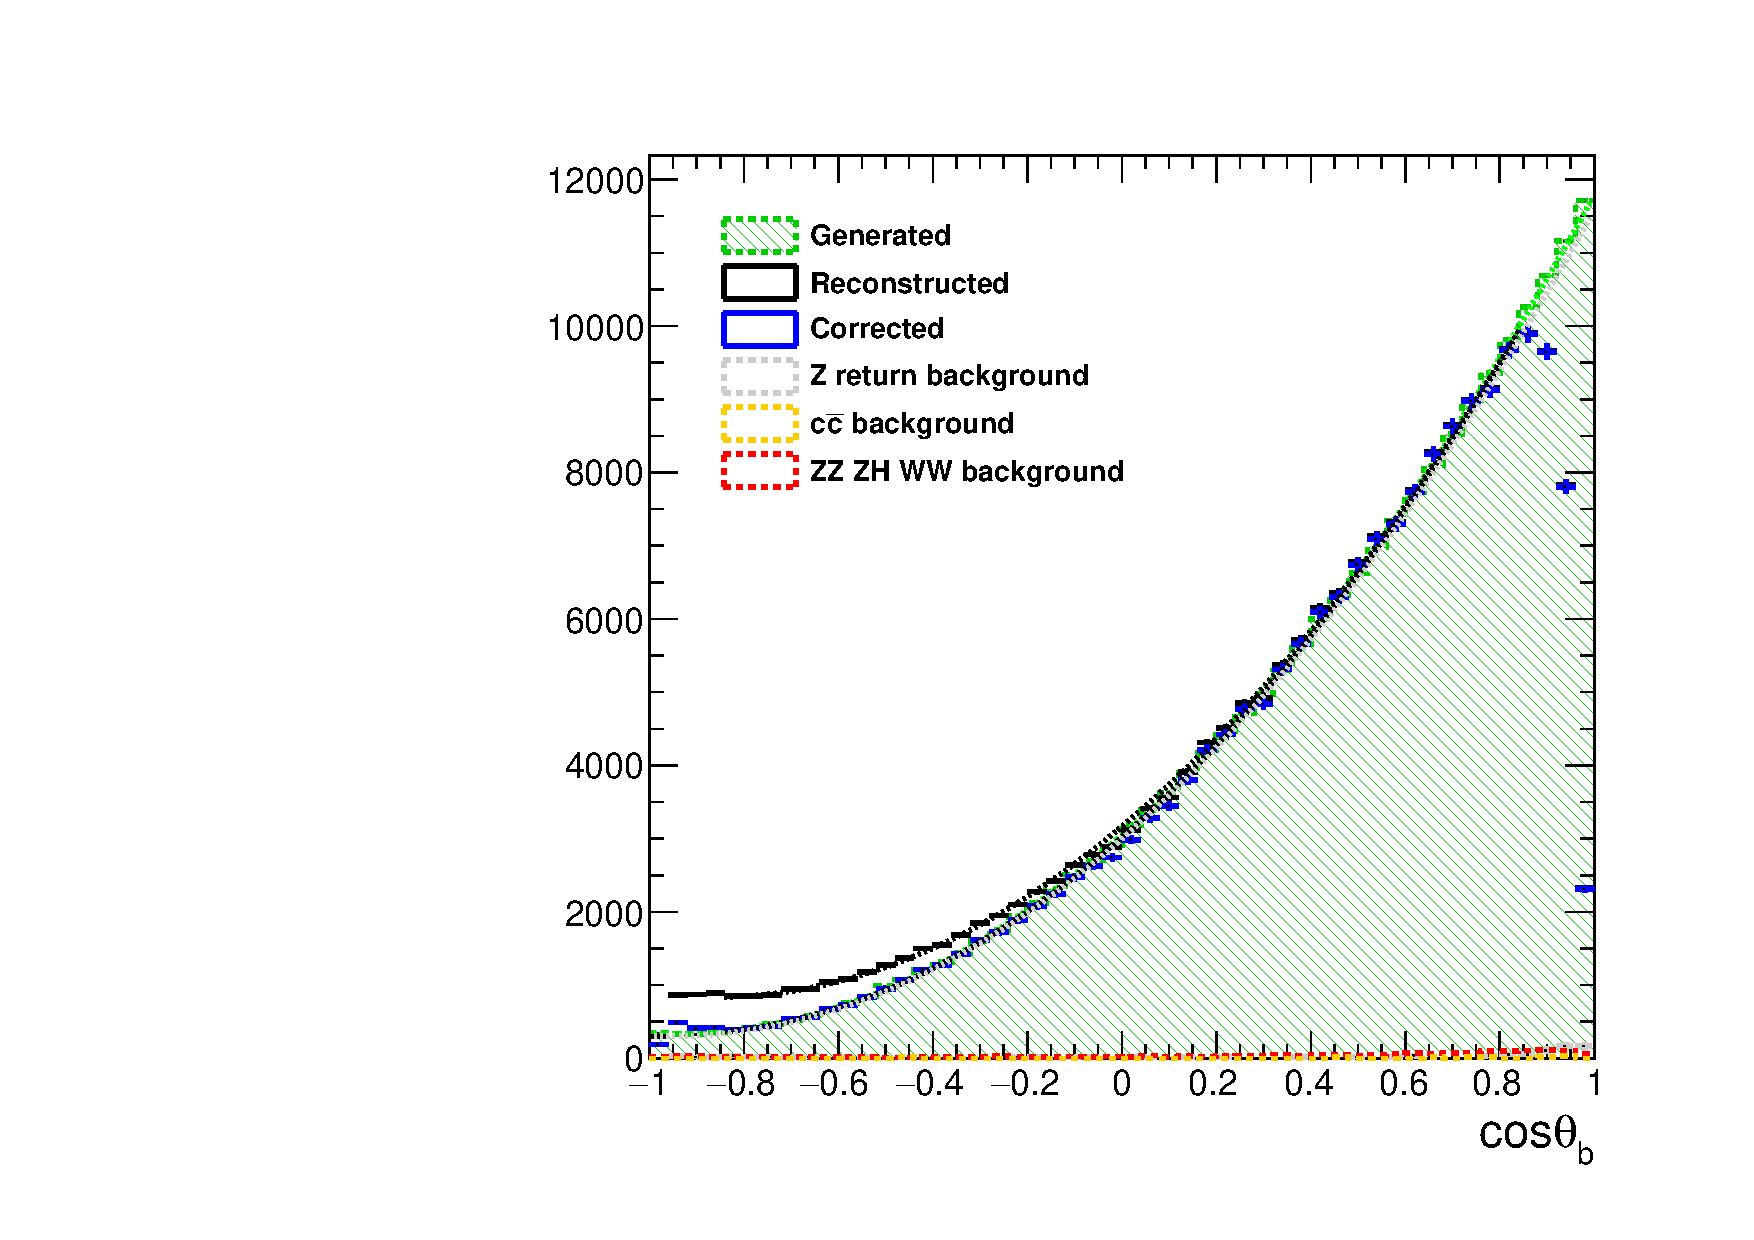
\includegraphics[width=0.95\textwidth]{ILD/plots/basymmetry-final-left.pdf}
		\llap{\shortstack{%
				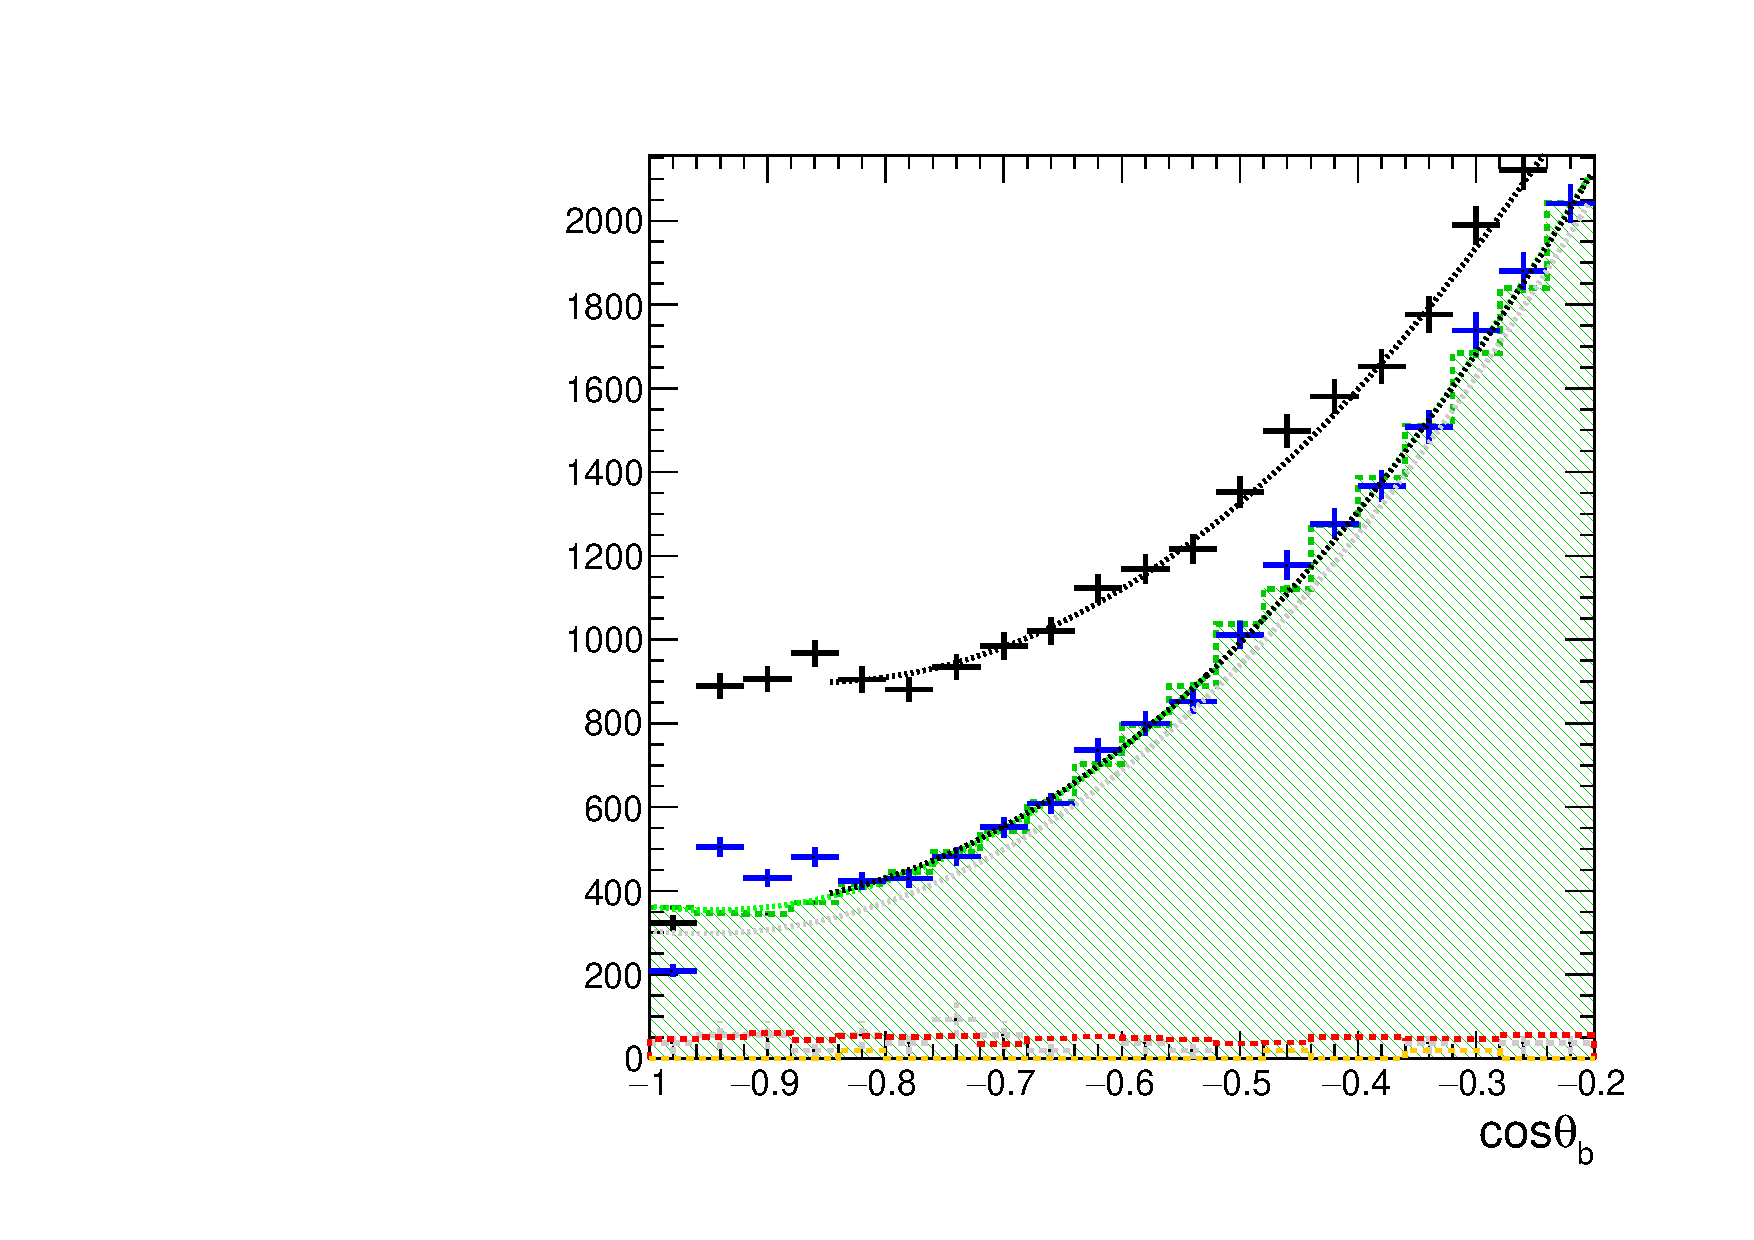
\includegraphics[clip, trim=0cm 0cm 1.8cm 1.7cm, scale=.14]{ILD/plots/zoom-final.pdf}\\
				\rule{0ex}{0.38in}%
			}
			\rule{1.8in}{0ex}}
		\caption{\label{fig:BAsymmetryFinal_a_3F} }
	\end{subfigure}% 
	\begin{subfigure}{0.5\textwidth}
		\centering
		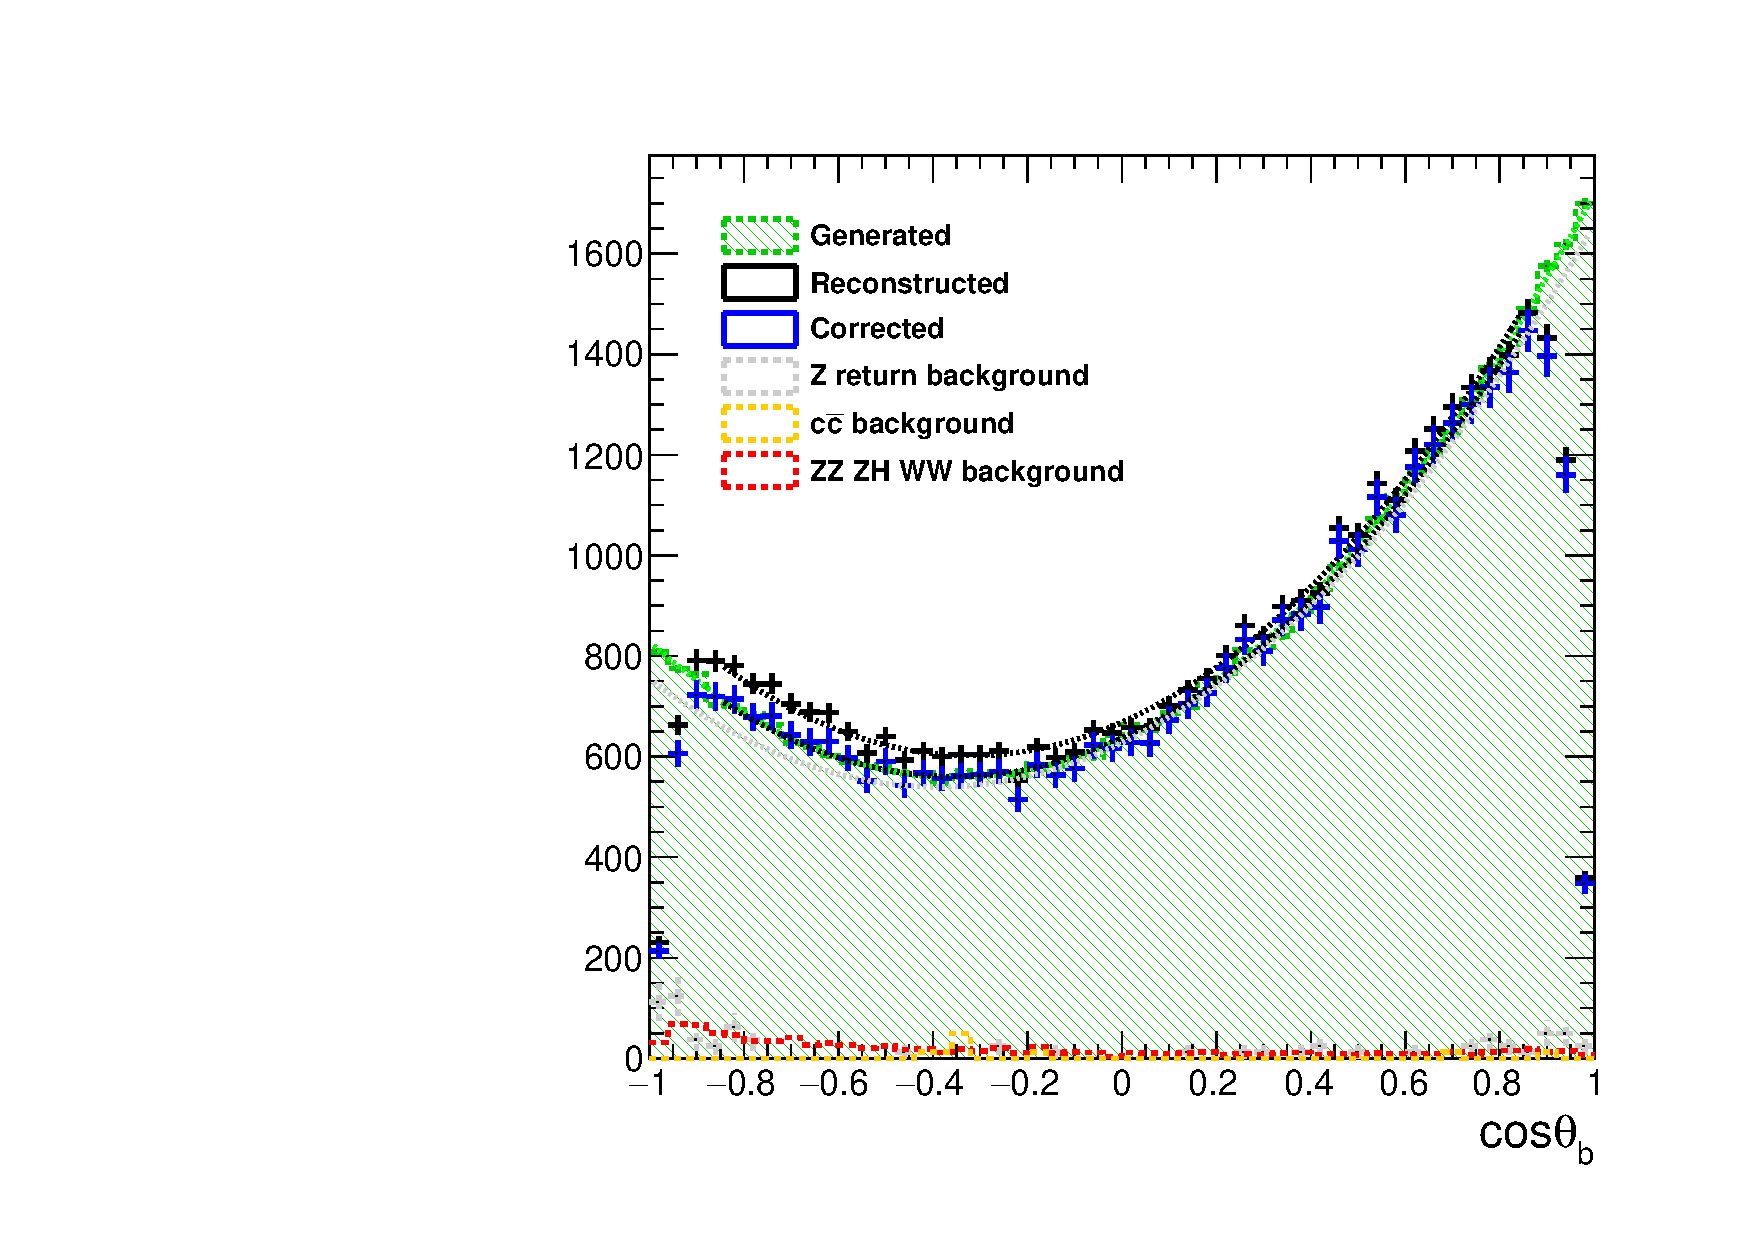
\includegraphics[width=0.95\textwidth]{ILD/plots/basymmetry-final-right.pdf}
		\caption{\label{fig:BAsymmetryFinal_b_3F} }
	\end{subfigure}
	\caption{\sl Generated b-quark polar angle distribution compared to the final reconstructed b-quarks polar angle in left-handed case (a) and right-handed case (b) with overlaid background processes.  }
	\label{fig:BAsymmetryFinal_3F}
\end{figure}



\begin{figure}
	\centering
	\begin{subfigure}{0.5\textwidth}
		\includegraphics[width=0.99\textwidth]{ILD/plots/lep-result-zoom.pdf}
		\caption{\label{fig:LEPILCResult_a_3F} }
	\end{subfigure}% 
	\begin{subfigure}{0.5\textwidth}
		\centering
		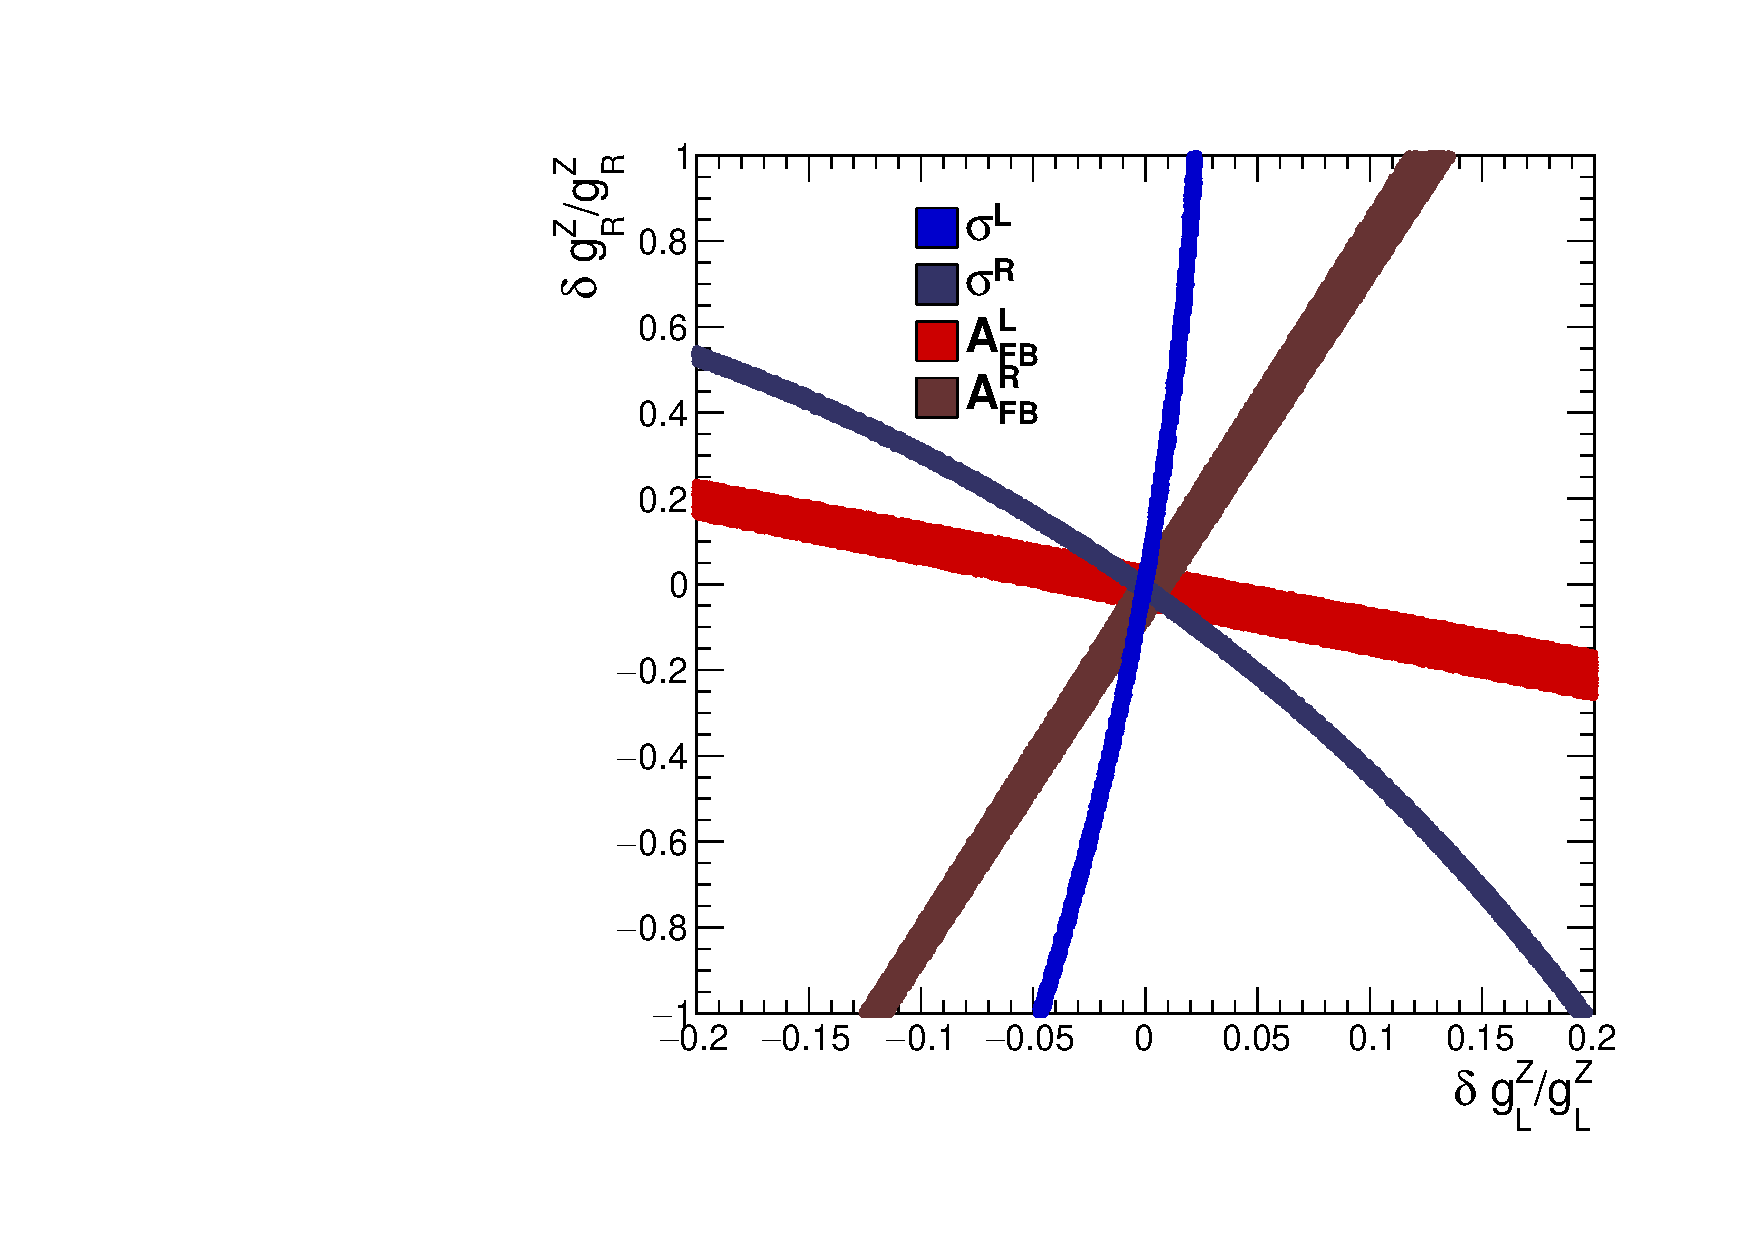
\includegraphics[width=0.99\textwidth]{ILD/plots/ilc-result.pdf}
		\caption{\label{fig:LEPILCResult_b_3F} }
	\end{subfigure}
	\caption{\sl Tree level $\pm 1\,\sigma$ allowed regions defined by the forward-backward asymmetry and total cross section measurements at LEP (a) and ILC via the differential cross section fit (b). Dashed guidelines show the \sm\ value. The allowed region expected at the ILC is centered at the \sm\ values of couplings.}
	\label{fig:LEPILCResult_3F}
\end{figure}







